\chapter{Development of Algorithms and Methodologies}
\label{sec:3}
In this chapter, all the new algorithms developed during the course of this work for the estimation of snow parameters from polarimetric SAR systems are explained. All the new methodologies are presented with detailed flowcharts and derivations. The detailed description about the study area, in-situ field data collection and the data sets used for this study are also incorporated in this chapter.

\section{Snow wetness estimation using dual polarimetric SAR data}
\label{sec:3.1}
In this section, a new snow wetness estimation method from dual-polarimetric coherent (HH/VV) SAR data
(i.e., TerraSAR-X) is developed which is based on the work of~\cite{jagdhuber2013polarimetric} for the estimation of soil moisture. In wet snow, the surface and the volume are the dominant scattering mechanisms. The snow surface wetness is estimated by using the simplified IEM model for high frequency limit of X-band (9.6 GHz) data. The snowpack volume wetness is estimated under the Rayleigh scattering assumption. The proposed method is used to estimate the snow wetness of the top layers ($\approx$ 15~cm) of the snowpack. 

The dual-polarimetric coherent TerraSAR-X data can be represented by a $2\times2$ coherency matrix ([$T_2$]) given in~(\ref{eq:coherency_matrix_dual}). In this study, we will analyze this coherency matrix to estimate the snow surface and the snow volume wetness. 
\begin{equation}
{
\mathbf{\langle[T_2]\rangle}= \frac{1}{2} \left[ \begin{array}{ccc}
<|S_{HH}+S_{VV}|^2> & <(S_{HH}+S_{VV})(S_{HH}-S_{VV})^*>\\
<(S_{HH}+S_{VV})^*(S_{HH}-S_{VV})> & <|S_{HH}-S_{VV}|^2>\\
\end{array}\right]	
 }
\label{eq:coherency_matrix_dual}
\end{equation}
In order to estimate the snow surface wetness, the simplified IEM scattering model is used to obtain the dominant scattering magnitude $(\alpha_1)$ under the high frequency limit of X-band (9.6 GHz)~\citep{allain2003}. The IEM model has been shown to be valid for a wide range of surface roughness~\citep{Fung92,fung1994microwave}. Usually a wet snow surface is rougher than a dry snow surface because of selective melting and re-freezing.  

A snow layer is an inhomogeneous medium composed of ice particles and water inclusions of different shapes, sizes, and orientations~\citep{Shi95wetness}. At a given sensor frequency, the snow density and the liquid water content affect the permittivity of snow. The Rayleigh scattering assumption has been used for the study of snowpack volume wetness, where the particles of the medium are considered substantially smaller than the incident wavelength. Finally, the effective snow wetness is obtained by suitably weighing the surface and the volume snow wetness components. The weights are obtained from the eigen-decomposition of the [$\mbox{T}_2$] matrix.

The in-situ measurements were obtained synchronously with the TerraSAR-X pass in January. Snow wetness measurements were taken at every 5~cm depth of the standing snow. The average wetness measurement is considered as the effective snow wetness which is then used to validate the results obtained from the proposed method.

\subsection{Snow surface wetness}
The dominant polarimetric scattering angle $(\alpha_1)$, corresponding to the dominant eigenvector and the eigenvalue is obtained from the dual coherent [$T_2$] matrix as shown in~(\ref{eq:alphas}).
\begin{equation}
\begin{split}
[T_2] &= [U_2][\Sigma][U_2]^{T} \\
U_2 &= \left[ \begin{array}{ccc}
u_{11} & u_{12} \\
u_{21} & u_{22} \\
\end{array} \right] \\
\alpha_1 &= \cos ^{ - 1}(|u_{11}|) 
\end{split}
\label{eq:alphas}
\end{equation}
where $[U_2]$ is a 2$\times$2 unitary matrix of the eigenvectors, $[\Sigma]$ is a $2\times2$ diagonal matrix of the eigenvalues and the superscript $T$ denotes matrix transpose. In the high frequency limit, like X-band (9.5 GHz), the dominant polarimetric scattering angle $(\alpha_1)$ obtained from the dual-polarimetric data is compared with the scattering angle $(\alpha_{IEM})$ estimated from the simplified IEM model for high frequency $(\nu)$ limit of X-band data ~(\ref{eq:highfreq})~\citep{allain2003}. 
\begin{equation}
\alpha_1 \approx \lim\limits_{\nu \rightarrow High}(\alpha_{IEM}) 
\label{eq:highfreq}
\end{equation}
The estimated $(\alpha_{IEM})$ from the simplified IEM model is only a function of the local incidence angle ($\theta$) and the surface dielectric constant $(\varepsilon_s)$ and is independent of the terrain roughness~(\ref{eq:iemalpha}). The local incidence angle $(\theta)$ is obtained using an external DEM (e.g. SRTM DEM).
\begin{equation}
\begin{split}
\lim\limits_{\nu \rightarrow High} (\alpha_{IEM}) &= \atan\left( \frac{2f_{hh}f_{vv}^{*}-X}{2f_{hh}f_{vv}^{*}+X}\right) \\
X = \left|f_{vv}\right|^2 - \left|f_{hh}\right|^2 + &\sqrt{\left(\left|f_{vv}\right|^2 - \left|f_{hh}\right|^2\right)^2 + 4\left|f_{hh}f_{vv}^{*}\right|^2}
\end{split}
\label{eq:iemalpha}
\end{equation}
The $f_{hh}=-\frac{2F_{hh}}{\cos\theta}$ and $f_{vv}=\frac{2F_{vv}}{\cos\theta}$ are the co-polarization scattering coefficients, where $F_{hh}$ and $F_{vv}$ are the Fresnel reflection coefficient for each polarization as a function of the local incidence angle $(\theta)$ and the dielectric constant $(\varepsilon_s)$. This estimated surface dielectric constant $(\varepsilon_s)$ is then used to compute the snow surface wetness using the Denoth's method $(W_s (\rho_d,\varepsilon_s))~\eqref{eq:denoth}~$~\citep{denoth1995electron}, where $\rho_d$ is the dry snow density.

\subsection{Snow volume wetness}
Apart from the snow surface wetness component, a small amount of snow volume wetness component is also expected with X-band data from a standing snow cover over ground since the penetration depth of the probing wave will be limited. The volume scattering of the snowpack is modeled as a random volume in this study. The snowpack particle structure shows high spatial variation and as a result of which it is difficult to model its volume scattering component. In this context, the particle anisotropy has been used to account for all snow particle structures. The anisotropy parameter which is interpreted in terms of the particle geometry is also characterized by the ratio of principal values of polarizability~\citep{cloude2009polarisation}. A random volume scattering coherency matrix is used in this study~(\ref{eq:volumemodel}) where $f_v$ is the volume scattering intensity and $A$ represents the particle anisotropy. 
\begin{equation}
\begin{split}
\frac{f_v}{(1+A^2)} \left[ \begin{array}{cc}
V_{11} & V_{12} \\
V_{12}^* & V_{22} \\
\end{array} \right]= \left[ \begin{array}{cc}
\frac{1}{2} & 0 \\
0 & \frac{1}{4} \\ 
\end{array} \right] \\
V_{11} = \frac{1}{2} (A+1)^2 ; V_{12} = 0 ;
V_{22} =\frac{1}{4}(A-1)^2 \\
\end{split}
\label{eq:volumemodel}
\end{equation}

The volume scattering intensity ($f_v$) is a function of the cross-polarization component ($S_{xx}$) in quad-polarimetric case. But, unlike in the quad-polarimetric data, the cross-polarization component is unavailable in the dual-polarimetric X-band $(\mbox{HH/VV})$ coherent data. Hence, this cross-polarization component is synthesized from the dual-polarimetric data under the azimuthally symmetric condition~(\ref{eq:crosspolestimation}).  
\begin{equation}
\begin{split}
f_v &= 8<|S_{xx}|^2> \\
<|S_{xx}|^2> &= \frac{1}{4} \left(1-\gamma_{HHVV}\right)\left(<|S_{HH}|^2>+<|S_{VV}|^2>\right) \\
\gamma_{HHVV} &= \frac{<S_{HH}S^*_{VV}>}{\sqrt{<|S_{HH}|^2><|S_{VV}|^2>}}
\end{split}
\label{eq:crosspolestimation}
\end{equation}
The quality of the estimated cross-polarization component cannot be assessed in this study due to the unavailability of a quad-polarimetric TerraSAR-X data along with the dual-polarimetric (HH/VV) coherent data. However, it has been shown that the Root Mean Square Error (RMSE) of the synthesized cross-polarization component for the TerraSAR-X data is around 1.8-2.0 dB compared to 5.0-5.4 dB for L-band E-SAR data over agricultural areas~\citep{Jagdhuber2014}. In this work our study area is a snow cover over flat bare ground devoid of any vegetation for which the condition of azimuthal symmetry can be assumed to be valid. By solving for the particle anisotropy $(A)$, it can be readily seen that it is a function of the volume scattering intensity $(f_v)$. In general the anisotropy parameter which is an indicator of particle shape is also bounded by the dielectric constant~(\ref{eq:anisotropy})~\citep{ablitt2000characterisation}. This dielectric constant is then used to estimate the volume snow wetness.
\begin{equation}
\frac{1}{\varepsilon_v} < A < \frac{\varepsilon_v + 1}{2}
\label{eq:anisotropy}
\end{equation}

In order to have an approximate estimate of $\varepsilon_v$, we have combined the lower and the upper bounds of the inequality involving the anisotropy parameter and $\varepsilon_v$. Any estimate of  $\varepsilon_v$ cannot lie below the curve given by $1/ A$ and below the line given by $2A-1$. An estimating function for $\varepsilon_v$ satisfying both these conditions is given by~(\ref{eq:volumedielctric}). As the value of the anisotropy parameter increases from 0 to 1, there is a rapid fall in the estimate of $\varepsilon_v$ as dictated by the lower bound. At $A=1$, the lower and the upper bounds of the inequality converge, and $\varepsilon_v$ is estimated as unity. Beyond this point there is a linear rise in the estimate of $\varepsilon_v$. 
\begin{equation}
\varepsilon_v = \frac{1}{A} + \left| \frac{1}{A} - (2A - 1)\right|
\label{eq:volumedielctric}
\end{equation}
\begin{equation}
W_e=
\begin{cases}
\bar{\lambda}_{1}W_s(\rho_d,\varepsilon_s) + \bar{\lambda}_{2}W_v(\rho_d,\varepsilon_v) \quad: W_s(\rho_d,\varepsilon_s) > W_v(\rho_d,\varepsilon_v) \\ 
\bar{\lambda}_{1}W_v(\rho_d,\varepsilon_v) + \bar{\lambda}_{2}W_s(\rho_d,\varepsilon_s) \quad: W_v(\rho_d,\varepsilon_v) > W_s(\rho_d,\varepsilon_s) \\
\end{cases}
\bar{\lambda}_{i} = \frac{\lambda_i}{\sum_{i=1,2}^{}\lambda_i}, \quad
\bar{\lambda}_{1} > \bar{\lambda}_{2}
\label{eq:effectivewetness}
\end{equation}
Similar to the snow surface wetness estimation, the volume dielectric constant $\varepsilon_v$ is used to estimate the snow volume wetness using the Denoth's method $(W_v (\rho_d,\varepsilon_v))$~\eqref{eq:denoth}, where $\rho_d$ is the dry snow density as used before. The effective snow wetness $(W_e)$ is estimated as a weighted average of the surface and the volume snow wetness according to~(\ref{eq:effectivewetness}). The pseudo probabilities computed from the eigenvalues are used to weigh $W_s(\rho_d,\varepsilon_s)$ and $W_v(\rho_d,\varepsilon_v)$ to estimate $W_e$. In the high frequency limit for the wet snow cover condition ($W_s(\rho_p,\varepsilon_s) > W_v(\rho_d,\varepsilon_v)$), the surface scattering is mostly the dominant scattering mechanism. Owing to this criteria, the surface wetness $W_s(\rho_d,\varepsilon_s)$ is weighted with the first dominant eigenvalue, $\bar{\lambda}_{1}$ and subsequently the volume wetness $W_v(\rho_d,\varepsilon_v)$ is weighted with the second dominant eigenvalue, $\bar{\lambda}_{2}$. In some cases (fairly less), when $W_v(\rho_d,\varepsilon_v) > W_s(\rho_d,\varepsilon_s)$, the volume wetness, $W_v(\rho_d,\varepsilon_v)$ is weighted with the first dominant eigenvalue, $\bar{\lambda}_{1}$ and the surface snow wetness, $W_s(\rho_d,\varepsilon_s)$ is weighted with the second dominant eigenvalue, $\bar{\lambda}_{2}$ to calculate the effective snow wetness $W_{e}$. The flowchart of the proposed snow wetness estimation methodology is shown in Figure~\ref{fig:flow_chart_sw_dual_pol}.
\begin{sidewaysfigure}[!htbp]
		\centering
		\includegraphics[width=0.6\columnwidth]{Figures_SW2/flow_chart}
		\caption [Flowchart of snow wetness estimation method for dual-pol data]{Flowchart of the proposed snow wetness estimation methodology.}
		\label{fig:flow_chart_sw_dual_pol}
\end{sidewaysfigure}	
\section{Snow wetness estimation using full polarimetric SAR data}
\label{sec:3.2}
In this section, a novel inversion model for the estimation of snow wetness from full-polarimetric SAR data is explained. This inversion technique is based on the G4U scattering power polarimetric decomposition technique. In wet snow, the surface and the volume are the dominant scattering mechanisms, therefore the generalized surface and the volume parameters are adopted. These parameters are then directly used to estimate the surface and the volume snow wetness. The effective snow wetness map is derived from the weighted average of both the wetness maps. The weights are derived from the normalized surface and volume scattering powers. 
\subsection*{Introduction}
The radar backscattering coefficient has been very useful for the quantitative estimation of snowpack parameters. Ground-based experiments were conducted to study the effect of dry and wet snow to backscattering coefficient of terrain~\citep{Stiles1980}. The measured backscattering coefficient is a function of several snow and soil parameters: snow layer, thickness, snow temperature, snow wetness, snow density, surface roughness (air-snow interface as well as snow-ground interface)~\citep{ulaby1986microwave}. Radar backscattering effects on geographical areas, relief, aspect angle, layover and shadow have also been studied~\citep{Koskinen97,Nagler2000,small2011flattening}. The snow volume scattering has been modeled by a discrete particle model which was experimentally justified at C-band~\citep{Kendra98,Koskinen2000}. A semi-empirical model for radar backscattering coefficient of snow covered ground was developed at 35~GHz and 95~GHz frequencies~\citep{Ulaby95}. This model relates the backscatter coefficient to the incidence angle and the snow-pack parameters (snow depth, crystal size and liquid water content) for each linear polarization.  

Several models have been developed to predict backscattering from rough surfaces: (1). the physical optics model, (2). the geometric optics model, (3). the small perturbation models (SPMs) and (4) the integral equation model (IEM) which is valid for a wide range of surfaces~\citep{Fung92,fung1994microwave}. Possibly due to surface roughness, several studies have shown both positive and negative correlation between the backscatter coefficient and snow wetness~\citep{stiles1980dielectric,shi1992radar}. Several algorithms for snow covered area retrieval have observed a negative correlation between the backscatter coefficient and wetness values for reasonable snow wetness and depth~\citep{Koskinen97,Nagler2000,Guneriussen2001b}. A inversion model has been developed to estimate snow wetness based on the first-order scattering model considering both surface and volume scattering~\citep{Shi93}. The NASA/JPL airborne AIRSAR imaging polarimetric data was used in this study. However, the first-order scattering model does not fit to most natural surfaces as they are very rough on the radar wavelength scale. The Integral Equation Model (IEM) which is valid over a wider range of surface roughness is used for the inversion model to estimate snow wetness~\citep{Shi95wetness}. The polarimetric space-borne Shuttle Imaging Radar Mission C-band (SIR-C) data was used for this study. The above method was modified to estimate snow wetness from conventional dual-polarization ENVISAT-ASAR data~\citep{singh2010snow}. A statistical inversion model was also developed to retrieve snow wetness using ENVISAT-ASAR alternating polarization data~\citep{niang2007new}. Recently, a new snow wetness estimation methodology has been proposed which utilizes the full-polarimetric SAR decomposition technique~\citep{Surendar13a}. 

A major advancement was made with the orientation compensation application in model-based polarimetric decompositions. This was necessary because of the fact that a target with different orientations in the plane orthogonal to the radar line of sight (LOS) will have different polarimetric responses. A number of decomposition methods with orientation compensation have been proposed to alleviate this issue~\citep{Lee2011,An10,YAMAGUCHI2011,singh13,arii2011adaptive,Chen14}. In the context of this work, the orientation compensation on the coherency matrix is important because of the gentle to very steep slopes of the Himalayan topography. These slopes vary in azimuth as well as in the range direction due to which there is an appreciable distortion in the backscattering observed in the Himalayan region as compared to horizontal flat surfaces. The polarization orientation shift or equivalently the cross-~polarization component is induced due to the azimuthally sloped surfaces~\citep{Lee2000,Lee2002}. In addition, the amount of the induced polarization orientation shifts is also a function of the radar look angle and the slope angle in the range direction. These effects in highly topographically irregular surfaces can be reduced with the help of polarization orientation compensation or minimization of the cross-polarized component. 

The Yamaguchi four-component decomposition with rotation of the coherency matrix (Y4R)~\citep{YAMAGUCHI2011} is the most frequently used method in SAR polarimetry. The Himalayan topography with gentle to steep slope behave like oriented surface from the radar illumination direction which causes the overestimation of the volume scattering component in the original Yamaguchi decomposition method (Y4O)~\citep{Yamaguchi2005}. The modified method (Y4R) compensates for the orientation changes along the radar line of sight which consequently decreases the volume scattering power. In this work we have used the general four-component scattering power decomposition method (G4U)~\citep{singh13} which is implemented by a double unitary transformation of the coherency matrix~(\ref{eq:g4u_decomposition_1} and~\ref{eq:g4u_decomposition_2}), 

\begin{subequations}
	\begin{multline}
	\left\langle\mathbf{[T(\theta)]}\right\rangle = \left[U(\theta)\right]\Bigl(f_{s}\left\langle\mathbf{[T]}\right\rangle_{surface} +  f_{d}\left\langle\mathbf{[T]}\right\rangle_{double} + f_v\left\langle\mathbf{[T]}\right\rangle_{vol} \\ + f_{c}\left\langle\mathbf{[T]}\right\rangle_{helix}\Bigr)\left[U(\theta)\right]^{\dagger}
	\label{eq:g4u_decomposition_1}
	\end{multline}
	\begin{equation}
	\left\langle\mathbf{[T(\phi)]}\right\rangle = \left[U(\phi)\right]\left\langle\mathbf{[T(\theta)]}\right\rangle\left[U(\phi)\right]^{\dagger} = \left[ \begin{array}{ccc}
	T_{11} & T_{12} & T_{13} \\
	T_{21} & T_{22} & 0 \\
	T_{31} & 0 & T_{33}
	\end{array}\right] 
	\label{eq:g4u_decomposition_2}
	\end{equation}
	\begin{equation}
	\left[U(\theta)\right] = \left[ \begin{array}{ccc}
	1 & 0 & 0 \\
	0 & \mbox{cos}2\theta & \mbox{sin}2\theta \\
	0 & -\mbox{sin}2\theta & \mbox{cos}2\theta
	\end{array}\right];  \quad
	\left[U(\phi)\right] = \left[ \begin{array}{ccc}
	1 & 0 & 0 \\
	0 & \mbox{cos}2\phi & j\mbox{sin}2\phi \\
	0 & j\mbox{sin}2\phi & \mbox{cos}2\phi
	\end{array}\right]
	\label{eq:utheta_and_uphi}
	\end{equation}
\end{subequations}
where $\dagger$ denotes complex conjugation and transposition, $\left[U(\theta)\right]$ and $\left[U(\phi)\right]$ denotes the real and the complex unitary transformation matrices respectively~(\ref{eq:utheta_and_uphi}) and $\left\langle\mathbf{[T(\theta)]}\right\rangle = \left[U(\theta)\right]\left\langle\mathbf{[T]}\right\rangle\left[U(\theta)\right]^{\dagger}$ denotes the measured coherency matrix after real orientation compensation. The $f_{s}$, $f_d$, $f_v$ and $f_{c}$ are the corresponding scattering coefficients of the expansion matrices, $\left\langle\mathbf{[T]}\right\rangle_{surface}$, $\left\langle\mathbf{[T]}\right\rangle_{double}$, $\left\langle\mathbf{[T]}\right\rangle_{vol}$ and $\left\langle\mathbf{[T]}\right\rangle_{helix}$ respectively. These coefficients are then used to estimate the surface ($P_s$), double-bounce ($P_d$), volume ($P_v$) and the helix ($P_c$) scattering powers. 

The G4U decomposition fully utilizes the polarimetric coherency phase information provided by a full-polarimetric SAR data. Unlike the Freeman-Durden decomposition (FDD)~\citep{freeman98}, the Y4O and the Y4R decompositions, which only uses 55.5$\%$, 66.6$\%$ and 75$\%$ of the polarimetric phase information respectively, the G4U utilizes 100$\%$ of the polarimetric phase information. The G4U decomposition also employs an extended volume scattering model to discriminate volume scattering between dipole and dihedral scattering structures caused by the cross-polarization (HV) component.

In the existing G4U decomposition method the volume scattering from forest cover and vegetation canopy has been modeled as a cloud of randomly oriented dipoles. However, a generalized spheroidal shape of snow particles is considered in the extension of G4U to express the volume scattering model over the wet snowpack to achieve a precise results of wetness~\citep{singh2013b}. Microwave interaction with snow depends on the dielectric and geometrical properties of the object. In general, the backscattering coefficient of snow-covered terrain consists of contributions from: (1) backscattering from air-snow interface, (2) volume scattering from the snow layer, and (3) backscattering from the underlying ground surface~\citep{ulaby1986microwave}. For wet snow, the important backscattering contributions result from the volume and the air-snow surface. The double-bounce scattering over snow covered terrain is small and hence can be neglected ($P_d\approx0$) ~\citep{singh2013b}.  

In this work the scattering by snow particles is modeled in terms of their polarizability. The volume scattering matrix defined for a single particle is defined as,
\begin{equation}
[S_{vol}]=\left[\begin{array}{cc}
S_{HH}^{vol} & 0 \\
0 & S_{VV}^{vol}
\end{array}\right] = S_{HH}^{vol}\left[\begin{array}{cc}
1 & 0 \\
0 & A_{p}
\end{array}\right]
\label{eq:scattering_matrix_fung_sw}
\end{equation}
where $A_{p}$ is known as the particle anisotropy. The anisotropy can also be interpreted in terms of the particle geometry and can be defined as the ratio of the principal values of polarizability~\cite{cloude2009polarisation}. In general, the anisotropy parameter can be used to a certain degree of reliability as a reference for the particle shape. However, the anisotropy parameter is also bounded by the dielectric constant ($\varepsilon$) of the particle and is bounded as shown in~\ref{eq:anisotropy},
In order to have a volume scattering from a random cloud of snow particles, the volume scattering matrix defined in~(\ref{eq:scattering_matrix_fung_sw}) should be arbitrarily rotated about the line of sight by an angle $\theta$ as,
\begin{equation}
[S_{vol}]=S_{HH}^{vol}\left[\begin{array}{cc}
\mbox{cos}(\theta) & \mbox{sin}(\theta) \\
-\mbox{sin}(\theta) & \mbox{cos}(\theta)
\end{array}\right]\left[\begin{array}{cc}
1 & 0 \\
0 & A_{p}
\end{array}\right]\left[\begin{array}{cc}
\mbox{cos}(\theta) & -\mbox{sin}(\theta) \\
\mbox{sin}(\theta) & \mbox{cos}(\theta)
\end{array}\right].
\label{eq:rotated_volume_scattering_matrix_sw}
\end{equation}
for which the volume coherency matrix $[T(\theta)]_{vol}$ can be written as,
\begin{equation}
[T(\theta)]_{vol}=\frac{1}{2}\left|S_{HH}^{vol}\right|^2\left[\begin{array}{ccc}
|1+A_{p}|^2 & (1 + A_{p})\mbox{cos}2\theta & -(1 + A_{p})\mbox{sin}2\theta    \\
(1 + A_{p})^*\mbox{cos}2\theta & |1-A_{p}|^2\mbox{cos}^22\theta  & -|1-A_{p}|^2\frac{\mbox{sin}4\theta}{2}   \\ 
-(1 + A_{p})^*\mbox{sin}2\theta & -|1-A_{p}|^2\frac{\mbox{sin}4\theta}{2} & |1-A_{p}|^2\mbox{sin}^22\theta
\end{array}\right].
\label{eq:coh_matrix_sp_sw}
\end{equation}
The volume scattering coherency matrix in~(\ref{eq:coh_matrix_sp_sw}) is averaged over all possible angles $\theta$ to obtain the volume scattering coherency matrix of a random cloud of small spheroid particles in one resolution cell as,
\begin{equation}
\left\langle[T]\right\rangle_{vol}^{snow}=\int[T(\theta)]_{vol}p(\theta)d\theta
\label{eq:average_coherency_matrix_sw}
\end{equation}
for uniformly distributed snow particles, 
\begin{equation}
p(\theta)=\frac{1}{2\pi} \quad; 0<\theta<2\pi
\label{eq:uniform_distrbn_sw}
\end{equation}
The average snow volume coherency matrix~(\ref{eq:volume_coherency_matrix_sw}) can be written in terms of generalized volume parameter ($|\gamma|^2$), 
\begin{equation}
\left\langle\mathbf{[T]}\right\rangle_{vol}^{snow} = f_{v}\left[ \begin{array}{ccc}
|\gamma|^{2} & 0 & 0 \\
0 & \frac{1}{2} & 0 \\
0 & 0 & \frac{1}{2}
\end{array}\right].
\label{eq:volume_coherency_matrix_sw}
\end{equation}
with the volume scattering coefficient as,
\begin{equation}
f_{v} = \frac{1}{2}|\gamma_{HH}-\gamma_{VV}|^{2}f(\theta_{i},\theta_{r},\omega,\tau,P)
\label{eq:fv_sw}
\end{equation}
where $\theta_{i}$ and $\theta_{r}$ are the local incidence and refractive angles, $\omega=\kappa_{s}/\kappa_{e}$ is the snow volume albedo, defined as the ratio of the scattering $\kappa_{s}$ and the extinction coefficient $\kappa_{e}$, $\tau$ is the optical depth ($\tau=\kappa_{e}d$) where $d$ is the snow depth, $P$ is the Rayleigh scattering phase function and,
\begin{equation}
|\gamma|^2 = \frac{|\gamma_{HH} + \gamma_{VV}|^2}{|\gamma_{HH} - \gamma_{VV}|^2} = \frac{|1 + A_{p}|^2}{|1 - A_{p}|^2}.
\label{eq:gammasquare_sw}
\end{equation}
where $\gamma_{HH}$ and $\gamma_{VV}$ are the Fresnel transmission coefficients for HH and VV polarizations respectively,
\begin{subequations}
	\begin{align}
	\gamma_{HH} =& \frac{2\sqrt{\varepsilon_{v} - \mbox{sin}^2\theta_{i}}}{\mbox{cos}\theta_{i} + \sqrt{\varepsilon_{v} - \mbox{sin}^2\theta_{i}}} \\
	\gamma_{VV} =& \frac{2\sqrt{\varepsilon_{v} - \mbox{sin}^2\theta_{i}}}{\varepsilon_{v}\mbox{cos}\theta_{i} + \sqrt{\varepsilon_{v} - \mbox{sin}^2\theta_{i}}}
	\end{align}
	\label{eq:fresnel_trans_coefficients_sw}
\end{subequations}
the local incidence angle $\theta_{i}$ should be converted into the local refractive angle $\theta_{r}$ using the Snell's law.
%Since $A_{p}$ is bounded, therefore $|\gamma|^2$ is also bounded as,
%\begin{equation}
%\left|\frac{\varepsilon_{v}+1}{\varepsilon_{v}-1}\right|^2 < |\gamma|^2 < \left|\frac{\varepsilon_{v}+3}{\varepsilon_{v}-1}\right|^2
%\end{equation}
By assuming that the double-bounce scattering is negligible in wet snow, the generalized volume parameter $|\gamma|^2$ is derived~\cite{singh2013b} as,
\begin{equation}
|\gamma|^2 = \frac{T_{11}(\theta)}{2T_{33}(\theta)-f_c} - \frac{|T_{12}(\theta)+T_{13}(\theta)|^{2}}{(2T_{33}(\theta)-f_{c})(T_{22}(\theta)-T_{33}(\theta)}
\label{eq:gamma_square_coherency_elememts_sw}
\end{equation}
where $f_{c}$ is the helix scattering coefficient given by,
\begin{equation}
f_{c}=2|\mbox{Im}\{T_{23}(\theta)\}|.
\label{eq:helix_scattering_coefficient_sw}
\end{equation}
The snow volume dielectric constant is then estimated by equating~(\ref{eq:gammasquare_sw}) and~(\ref{eq:gamma_square_coherency_elememts_sw}).   

\begin{sidewaysfigure}[!htbp]
		\centering
		\includegraphics[width=0.85\columnwidth]{Figures/flow_chart_1}
		\caption{Flowchart of the proposed methodology for snow wetness estimation using full polarimetric SAR data.}
		\label{fig:fullpol_methodology}
\end{sidewaysfigure}

In a similar way, the average snow surface coherency matrix is given as,
\begin{equation}
\left\langle\mathbf{[T]}\right\rangle_{surface}^{snow} = f_{s}\left[ \begin{array}{ccc}
1 & \beta^* & 0 \\
\beta & |\beta|^{2} & 0 \\
0 & 0 & 0
\end{array}\right] 
\label{eq:surface_coherency_matrix_sw}
\end{equation}
with the surface scattering coefficient as,
\begin{equation}
f_s=\frac{1}{2}|\alpha_{HH} + \alpha_{VV}|^2f(\theta_{i},s,\bm{k})W
\label{eq:fs_sw}
\end{equation}
where $s$ is the snow rms height, $\bm{k}$ is the wave number, $W$ is the Fourier transform component of the surface correlation length and,
\begin{equation}
|\beta|^2 = \left|\frac{\alpha_{HH}-\alpha_{VV}}{\alpha_{HH}+\alpha_{VV}}\right|^2
\label{eq:betasquare_sw}
\end{equation}
where $\alpha_{HH}$ and $\alpha_{VV}$ are the Bragg coefficients for HH and VV polarizations respectively.  
\begin{subequations}
	\begin{align}
	\alpha_{HH} =& \frac{\mbox{cos}\theta_{i} - \sqrt{\varepsilon_{s} - \mbox{sin}^2\theta_{i}}}{\mbox{cos}\theta_{i} + \sqrt{\varepsilon_{s} - \mbox{sin}^2\theta_{i}}} \\
	\alpha_{VV} =& (\varepsilon_{s}-1)\frac{\mbox{sin}^2\theta_{i} - \varepsilon_{s}(1 + \mbox{sin}^2\theta_{i})}{\left[\varepsilon_{s}\mbox{cos}\theta_{i} + \sqrt{\varepsilon_{s} - \mbox{sin}^2\theta_{i}}\right]^2}.
	\end{align}
	\label{eq:fresnel_refl_coefficients_sw}
\end{subequations}
The generalized surface parameter $|\beta|^2$ is derived from the coherency matrix~\citep{singh2013b} as,
\begin{equation}
|\beta|^2 = \left|\frac{T_{12}(\theta) + T_{13}(\theta)}{T_{11}(\theta) - f_{v}|\gamma|^2}\right|^2
\label{eq:beta_square_coherency_elememts_sw}
\end{equation}
where $|\gamma|^2$ is the generalized volume parameter derived above.
The snow surface dielectric constant is then estimated by equating~(\ref{eq:betasquare_sw}) and~(\ref{eq:beta_square_coherency_elememts_sw}). The snow surface and the volume dielectric constants are used in the empirical equation~(\ref{eq:wetness})~\citep{denoth1995electron} to estimate the snow surface and the volume wetness. 
\begin{equation}
W(\%) = 5.35[\varepsilon -(1+1.92\rho)]
\label{eq:wetness}
\end{equation} 
The effective snow wetness ($W_e$)~(\ref{eq:effective_snow_wetness}) is derived from the surface ($W_s$) and the volume ($W_v$) snow wetness using the corresponding scattering powers ($P_S$ and $P_v$) derived from the G4U decomposition for snow, 
\begin{equation}
W_e(\%) = \omega_{s}W_{s} + \omega_{v}W_{v}; \quad \omega_{s}+\omega_{v}=1
\label{eq:effective_snow_wetness}
\end{equation}
where $\omega_{s}=\frac{P_s}{P_s+P_v}$ and $\omega_{v}=\frac{P_v}{P_s+P_v}$. The flowchart of the proposed methodology is shown in Figure~\ref{fig:fullpol_methodology}.
\begin{figure*}[!h]
	\centering
	\includegraphics[width=0.6\textwidth]{Figures/plot}
	\caption[Plot of Snow wetness Vs Penetration depth at C-band]{Penetration depth as a function of snow wetness at C-band microwave frequency.}
	\label{fig:penetration_plot}
\end{figure*}

The C-band microwave signal will approximately penetrate 5--20~cm when the snowpack has liquid water content of $< 4\%$ by volume as can be very well observed in Figure~\ref{fig:penetration_plot}. For saturated snow wetness ($> 8\%$ by volume), the penetration depth is only a few millimeters. It is understandable that snowpack wetness will vary depending on the condition of snow on the ground. For snow surface melt condition, the surface scattering power will be higher than the snowpack volume scattering power. So in this case, the effective wetness will have more percentage of surface wetness contribution than the snowpack volume wetness. On the other hand, in dry snow condition, (eg., during snow fall) the snowpack is completely dry within few centimeters (depending on the duration and condition of snowfall) while the volume may have higher wetness due to the older snowpack. In this condition, the effective snow wetness will have more percentage of volume wetness contribution than the surface wetness.

\section{Estimation of snow surface dielectric constant from polarimetric SAR data}
\label{sec:3.3}
In this section, a new method to estimate snow surface dielectric constant from polarimetric SAR data is explained. The novelty of the method is realized by the introduction of the effective degree of polarization estimated by unitary rotation of the coherency matrix. This technique leads to maximize the number of surface scattering pixels for inversion.  A ratio of the Bragg coefficients $B_{HH}$ and $B_{VV}$ as a function of the local incidence angle $\theta_{i}$ and the dielectric constant $\varepsilon_{r}$ is related to the dominant scattering type magnitude $\alpha_{s1}$~\citep{TOUZI2007}. An inversion technique is then used to estimate the dielectric constant $\varepsilon_{r}$. A similar inversion approach is proposed in~\citep{Hajnsek2003} to invert soil surface parameters from polarimetric SAR data using the Cloude-Pottier entropy ($H$) and alpha ($\alpha$).

\subsection{Dominant scattering mechanism}
In this study, dominant scattering type amplitude is considered to characterize scattering of snow. In order to understand this it is very essential to know that which layers of snow/ice are primarily responsible for this scattering. The scattering from volume is mainly observed from dry snow in which microwaves can penetrate 10~m at 10~GHz~\citep{rott1987possibilities}. However, small variations in liquid water content in snow significantly reduces the penetration depth~\citep{rott1987possibilities,rott1995monitoring}. 

The dominant scattering type amplitude ($\alpha_{s1}$) is obtained from the eigenvalue/eigenvector based incoherent target decomposition (ICTD) theorem proposed in~\cite{TOUZI2007}. In general, ICTD is used to express the averaged scattering mechanism given by a $3\times3$ coherency matrix $\langle[{\mathbf{T}}]\rangle$ as a sum of independent scattering components~\citep{Cloude92NATO,Cloude96,TOUZI2007}. The $\alpha$--$\beta$ scattering model proposed in~\cite{Cloude96} differs from the scattering model proposed in~\cite{TOUZI2007} for non-symmetric targets. The scattering type parameter $\alpha$ introduced by Cloude-Pottier is in fact a function of the symmetric scattering type magnitude $\alpha_{s}$ and the helicity $\tau_{m}$. However, the dominant scattering type $\alpha_{s1}$ obtained from the first eigenvector (corresponding to $p_{1}$ with $p_{3}<p_{2}<p_{1}$, where $p_{i}=\lambda_{i}/\sum_{1}^{3}\lambda_{i}$) is similar to $\alpha_{1}$ for $\tau_{m}\simeq0$. In this study, while considering the dominant scattering type from the snow surface, a subset $\alpha_{s1}^{B}$~\eqref{eq:alpha_subset} of $\alpha_{s1}$ has been considered which characterizes Bragg scattering. 
\begin{equation}
\alpha_{s1}^{B}=\Big\{\{\alpha_{s1} \in [0,90^\circ]: p_{1}\ge 0.7\} \le 20^\circ\Big\}
\label{eq:alpha_subset}
\end{equation}
Therefore, $\alpha_{s1} \in \alpha_{s1}^{B}$ has been considered for analysis in this study. The $\alpha_{s1}$ image of the study site for 8 Feb.2013 data is shown in Figure~\ref{fig:results_1}(c). It can be clearly seen that $\alpha_{s1} \le 20^\circ$ for most of the areas. Moreover, it can be seen that in the higher altitudes ($> 4000$~m.a.s.l) $\alpha_{s1} \ge 40^\circ$ which may be due to volume scattering from dry snowpack. 
%In the next section the effective (optimum) degree of polarization is estimated by unitary transformations of the coherency matrix. 

\subsection{Degree of polarization}
The degree of polarization ($m$) is defined as the ratio of the (average) intensity of the polarized portion of the wave to that of the (average) total intensity of the wave. For a completely polarized EM wave, $m = 1$ and for a completely unpolarized EM wave, $m = 0$. In between these two extreme cases, the EM wave is said to be partially polarized, $0 < m < 1$. In this study, two independent methods have been used to derive the optimum degree of polarization. In one method, the optimum degree of polarization is derived by unitary transformation (both real and complex) of the 3$\times$3 coherency matrix $\mathbf{\langle[T]\rangle}$ for which the cross-polarization component ($T_{33}$) is minimized. In another method, the optimum degree of polarization $(p_{max}~\mbox{and}~p_{min})$ is derived by numerically solving a sixth order polynomial equation formed by the elements of the Mueller matrix. The optimum degree of polarization obtained from these two methods is then compared for the estimation of the snow surface dielectric constant. 

\subsubsection{AGU pptimum degree of polarization (AGU--Dop)}
In some model-based decompositions the $3\times3$ multi-look coherency $\mathbf{\langle[T]\rangle}$ or the covariance $\mathbf{\langle[C]\rangle}$ matrices (where $\langle\dots\rangle$ denotes ensemble averaging) is rotated by a real matrix $[{\mathbf{R}}(\theta)]$~\eqref{eq:R_theta} about the radar line of sight (LOS). The angle $\theta$ is obtained by minimizing the $T_{33}(\theta)$ component of $\mathbf{\langle[T]\rangle}$: $\frac{\partial T_{33}(\theta)}{\partial \theta}=0$. 
\begin{equation}
[{\mathbf{R}}(\theta)] = \left[ \begin{array}{ccc}
1 &0 & 0 \\
0 & \cos(2\theta) & \sin(2\theta) \\
0 & -\sin(2\theta) & \cos(2\theta)
\end{array}\right] 
\label{eq:R_theta} 
\end{equation}
The fundamental idea behind such compensation is to minimize the cross-polarization component. The orientation compensation can be used to reduce the overestimation of the volume power in a model-based decomposition to a certain extent and increase the double-bounce power. 

In the proposed method~\citep{bhattacharya2015adaptive}, after the real rotation, two complex unitary transformation matrices $[{\mathbf{R}}(\phi_1)]$ and $[{\mathbf{R}}(\phi_2)]$~\eqref{eq:R_phi_2} were applied to the $\langle[{\mathbf{T}}(\theta)]\rangle$ matrix,
\begin{align*}
\langle[{\mathbf{T}}(\phi_1)]\rangle&=[{\mathbf{R}}(\phi_1)]\langle[{\mathbf{T}}(\theta)]\rangle[{\mathbf{R}}(\phi_1)]^{-1} \quad \mbox{and},\\[0.4em] 
\langle[{\mathbf{T}}(\phi_2)]\rangle&=[{\mathbf{R}}(\phi_2)]\langle[{\mathbf{T}}(\theta)]\rangle[{\mathbf{R}}(\phi_2)]^{-1}
\end{align*}
where the angles $\phi_{1}$ and $\phi_{2}$ are obtained similarly by minimizing the  $T_{33}(\phi_{1})$ and the $T_{33}(\phi_{2})$ components respectively: $\frac{\partial T_{33}(\phi_{1})}{\partial \phi_{1}}=0$ and $\frac{\partial T_{33}(\phi_{2})}{\partial \phi_{2}}=0$. 
\begin{gather}
[{\mathbf{R}}(\phi_1)] = \left[ \begin{array}{ccc}
1 & 0 & 0 \\
0 & \cos(2\phi_1) & j\sin(2\phi_1) \\
0 & j\sin(2\phi_1) & \cos(2\phi_1)
\end{array}\right] \label{eq:R_phi_1} \\[0.5em] 
[{\mathbf{R}}(\phi_2)] = \left[ \begin{array}{ccc}
\cos(2\phi_2) & 0 & j\sin(2\phi_2) \\
0 & 1 & 0 \\
j\sin(2\phi_2) & 0 & \cos(2\phi_2)
\end{array}\right] 
\label{eq:R_phi_2}
\end{gather}

In order to compute the degree of polarization, the coherency matrices $\langle[{\mathbf{T}}(\phi_1)]\rangle$ and $\langle[{\mathbf{T}}(\phi_2)]\rangle$ are transformed into a $4\times4$ Mueller matrices $\langle[{\mathbf{M}}(\phi_1)]\rangle$ and $\langle[{\mathbf{M}}(\phi_2)]\rangle$ respectively. The received Stokes vectors $\mathbf{G_{H}^{r}}=\begin{bmatrix} g_{H1}^{r} & g_{H2}^{r} & g_{H3}^{r} & g_{H4}^{r}
\end{bmatrix}^{T}$ and $\mathbf{G_{V}^{r}}=\begin{bmatrix}
g_{V1}^{r} & g_{V2}^{r} & g_{V3}^{r} & g_{V4}^{r}
\end{bmatrix}^T$ for a horizontal and a vertical  polarizations respectively are related to the
transmit Stokes vectors $\mathbf{G_{H}^{t}} = \begin{bmatrix}
1 & 1 & 0 & 0
\end{bmatrix}^T$ and $\mathbf{G_{V}^{t}} = \begin{bmatrix}
1 & {-1} & 0 & 0
\end{bmatrix}^T$ for linear horizontal and vertical polarizations respectively by $\mathbf{G_{H/V}^{r}}=\mathbf{\langle[M]\rangle}\mathbf{G_{H/V}^{t}}$. The degree of polarization of a received EM wave for a horizontally (H) and a vertically (V) transmitted wave is defined as $m_{H}$ and $m_{V}$~\eqref{eq:dop} respectively, and $m_{E}$ is the effective degree of polarization~\eqref{eq:dop_h_v}.
\begin{gather}
m_{H} = \frac{\Big(\sum_{i=2}^{4}({g_{Hi}^{r}})^2 \Big)^{1/2}}{g_{H1}^{r}},\quad\label{eq:dop}
m_{V} = \frac{\Big(\sum_{i=2}^{4}({g_{Vi}^{r}})^2 \Big)^{1/2}}{g_{V1}^{r}}\\[0.1em] 
m_{E} = \Bigg(\frac{m_{H}^{2}+m_{V}^{2}}{2}\Bigg)^{1/2}
\label{eq:dop_h_v}
\end{gather}

The two independent $m_{E}$'s which are obtained from the Mueller matrices, $\langle[{\mathbf{M}}(\phi_1)]\rangle$ and $\langle[{\mathbf{M}}(\phi_2)]\rangle$ are compared and the maximum among the two $m_{E}^{\mbox{\scriptsize opt}}$ is retained for that particular pixel as shown in Figure~\ref{fig:results_1}(a). Along with $\alpha_{s1} \in \alpha_{s1}^{B}$, the $m_{E}^{\mbox{\scriptsize opt}}$ is used to delineate the pixels which are then used to estimate the dielectric constant by an inversion technique.
%===============================================%
\subsubsection{Touzi optimum degree of polarization}
In~\cite{touzi1992polarimetric}, a new method have been developed to optimize the degree of polarization of a partially polarized wave. An analytical computation method has been developed to derive the optimum degree of polarization $(p_{max}~\mbox{and}~p_{min})$ along with the scattered wave intensity. This unique method is based on Lagrange multiplier which shows that the optimum degree of polarization $(p_{max}~\mbox{and}~p_{min})$ can be obtained by numerically solving a sixth order polynomial equation~\citep{touzi1992polarimetric}. This also leads to the estimation of the optimum polarization angles $(\chi_{t}^{\mbox{\scriptsize opt}},\psi_{t}^{\mbox{\scriptsize opt}})$. The optimum degree of polarization is derived using the elements of the Mueller matrix along with the $(\chi_{t},\psi_{t})$. The $\Delta p$ parameter (the deviation of the degree of polarization) along with the $p_{min}$ parameter has shown significant improvement in the ship-sea contrast compared to single polarization (HH, VV and HV) channels~\citep{Touzi2015}. The $p_{max}$ obtained for the 8 Feb 2013 Radarsat-2 data over the study area is shown in Figure~\ref{fig:results_1}(b).

\begin{figure*}[!h]
	\centering
	\subfloat[]{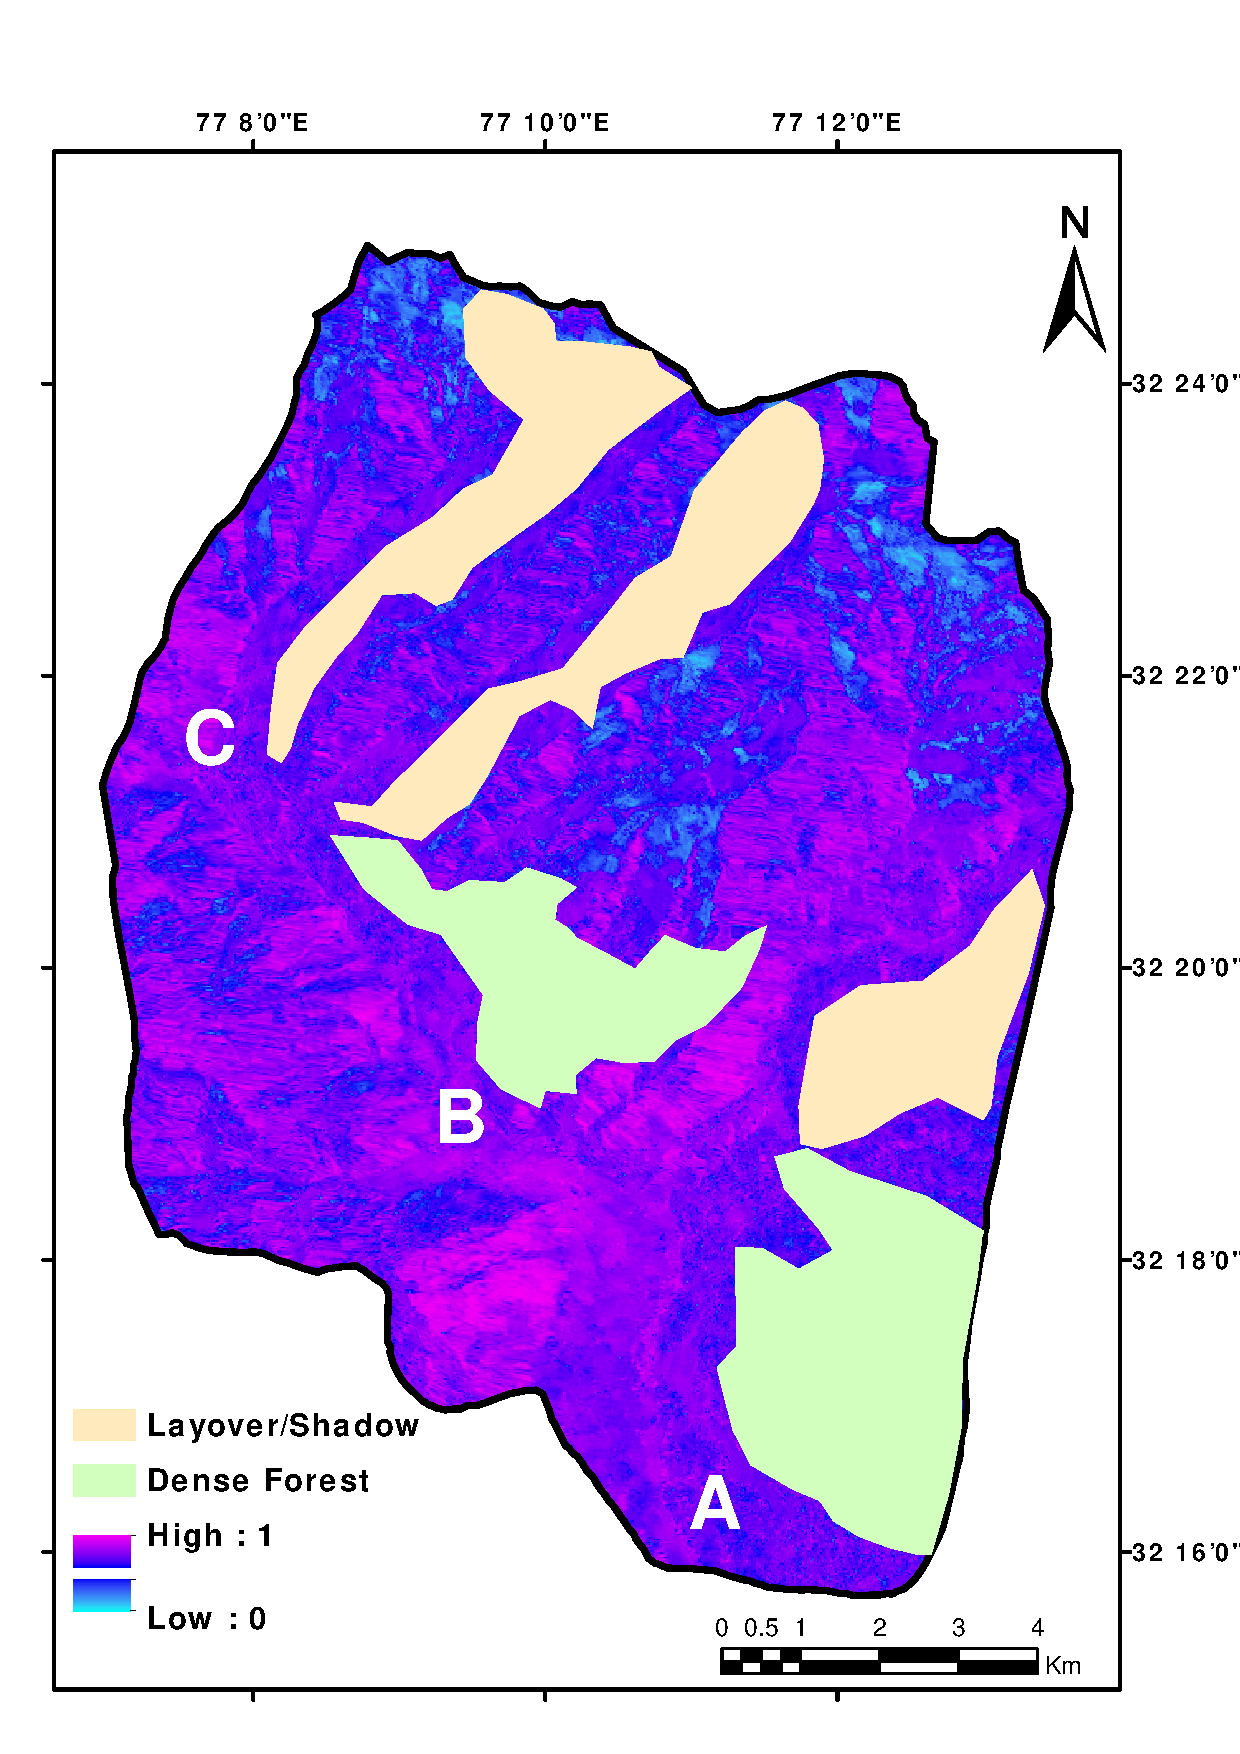
\includegraphics[width=0.4\columnwidth]{Figures_SSD/Ag4U_DOP}} 
	\hspace{1mm}
	\subfloat[]{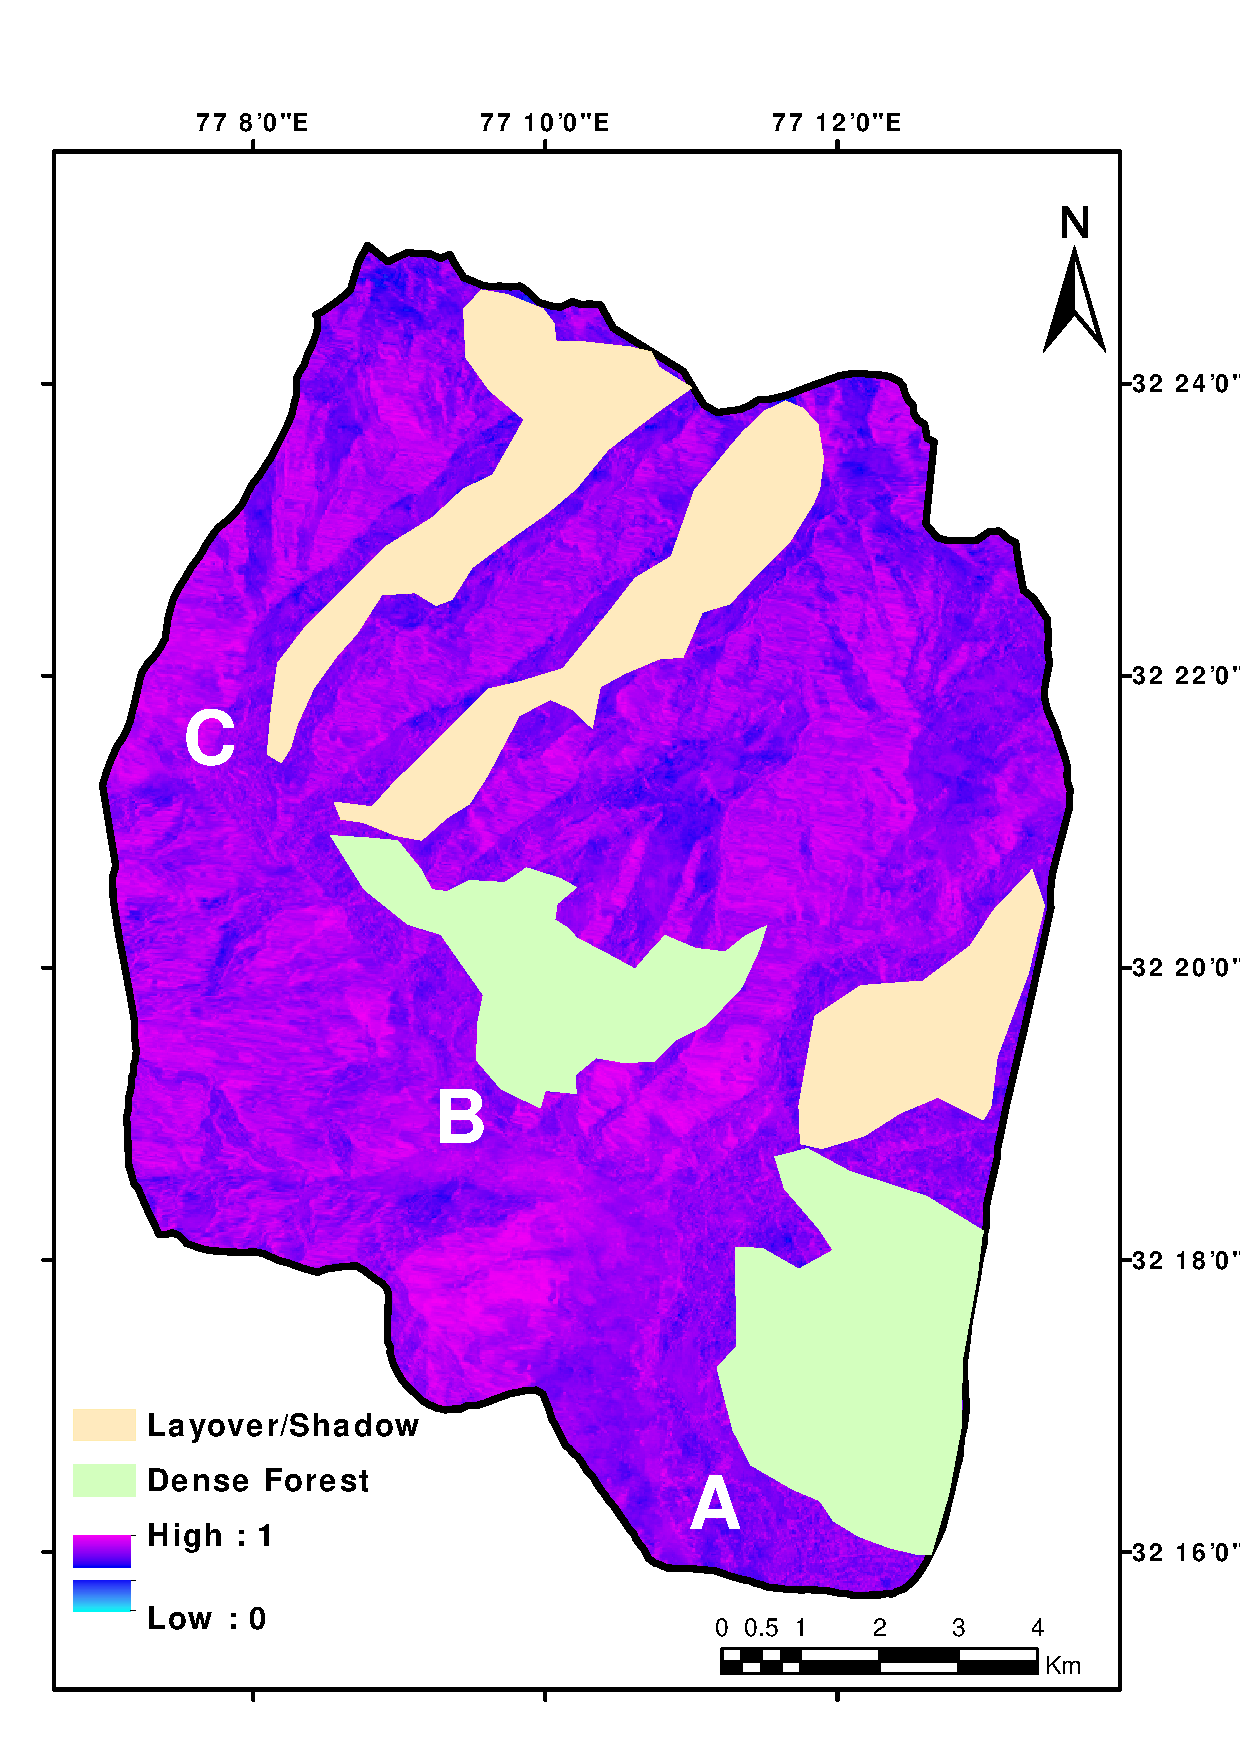
\includegraphics[width=0.4\columnwidth]{Figures_SSD/Touzi_DOP}} 
	\vspace{1mm}
	\subfloat[]{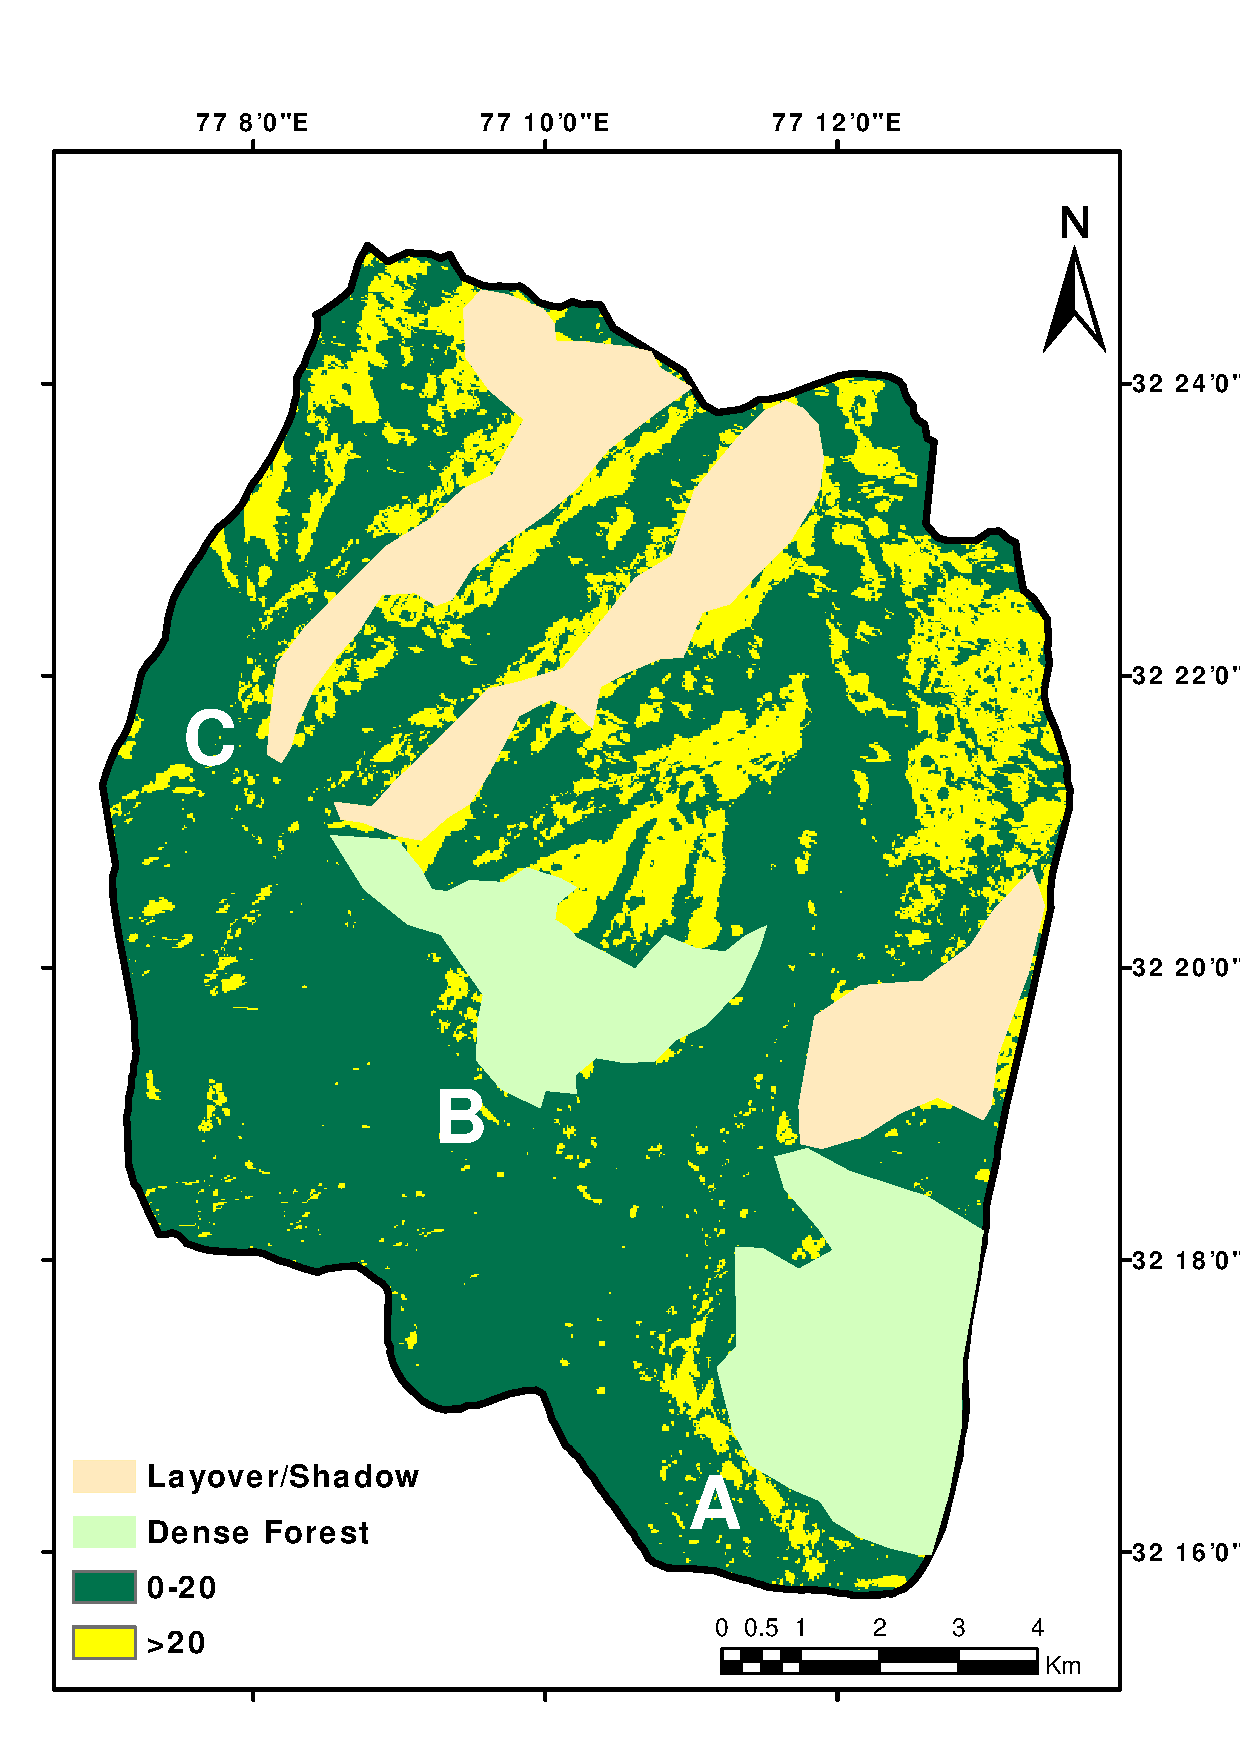
\includegraphics[width=0.4\columnwidth]{Figures_SSD/alpha_8feb13}} \hspace{1mm}
	\subfloat[]{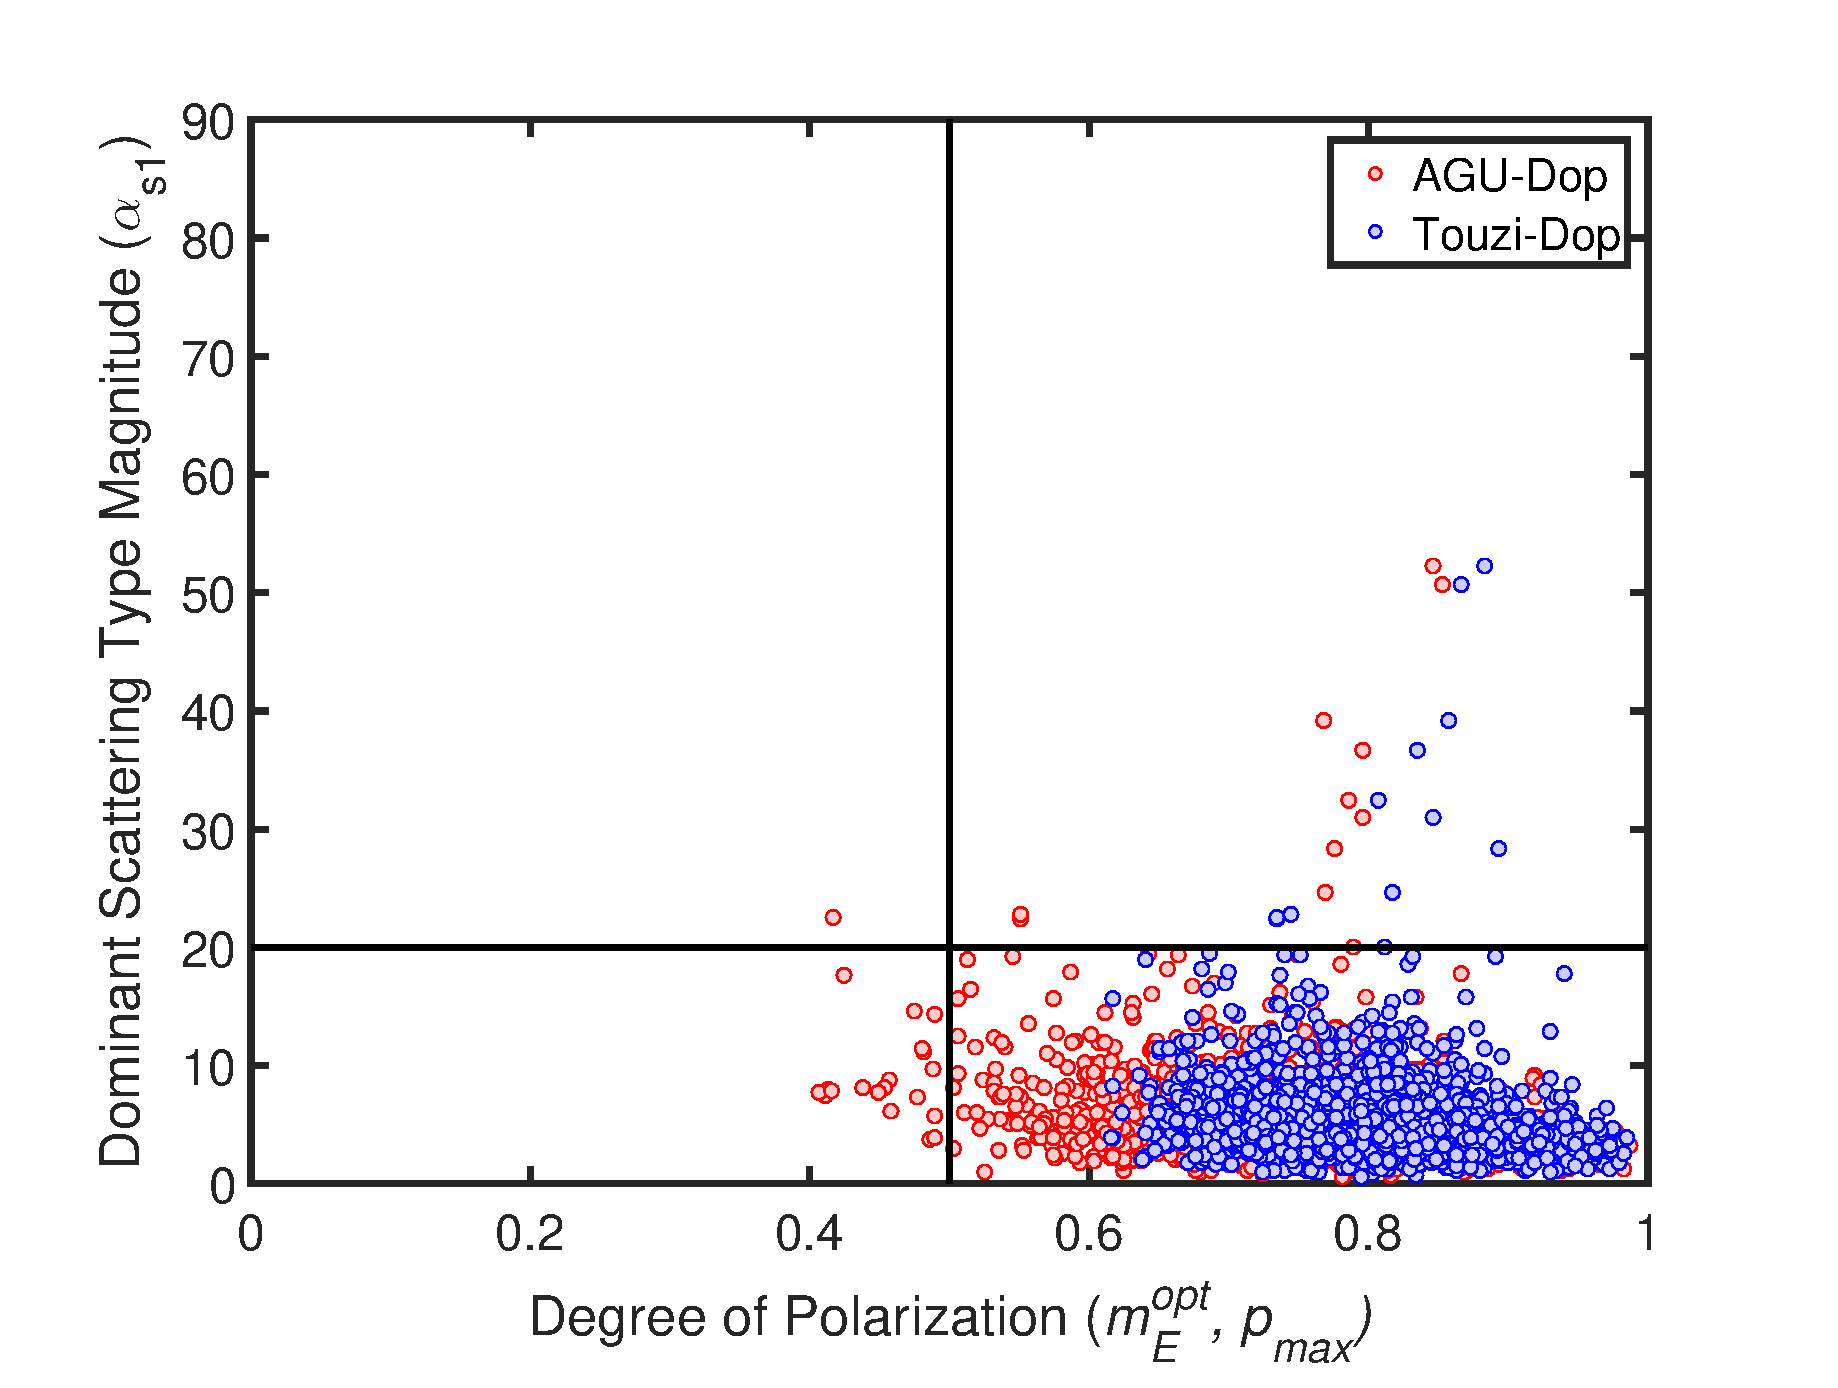
\includegraphics[width=0.4\columnwidth]{Figures_SSD/dop_alpha_1}} 
	\caption[The optimum degree of polarization by (a) AGU (b) Touzi methods, (c) the dominant scattering type magnitude and (d) the $\alpha_{s1} \mbox{vs.} m_{E}^{\mbox{\scriptsize opt}}$ plot for 8 Feb.2013 data]{The optimum degree of polarization by (a) AGU and (b) Touzi methods, (c) the dominant scattering type magnitude and (d) the $\alpha_{s1} \mbox{vs.} m_{E}^{\mbox{\scriptsize opt}}$ plot for 8 Feb.2013 data. The points A, B and C on the maps are the three observatory locations over the study area.}
	\label{fig:results_1}
\end{figure*}
%\begin{figure*}[!h]
%	\centering
%	\subfloat[$m_{E}^{\mbox{\scriptsize opt}}$\label{Fig:AGU_DOP}]{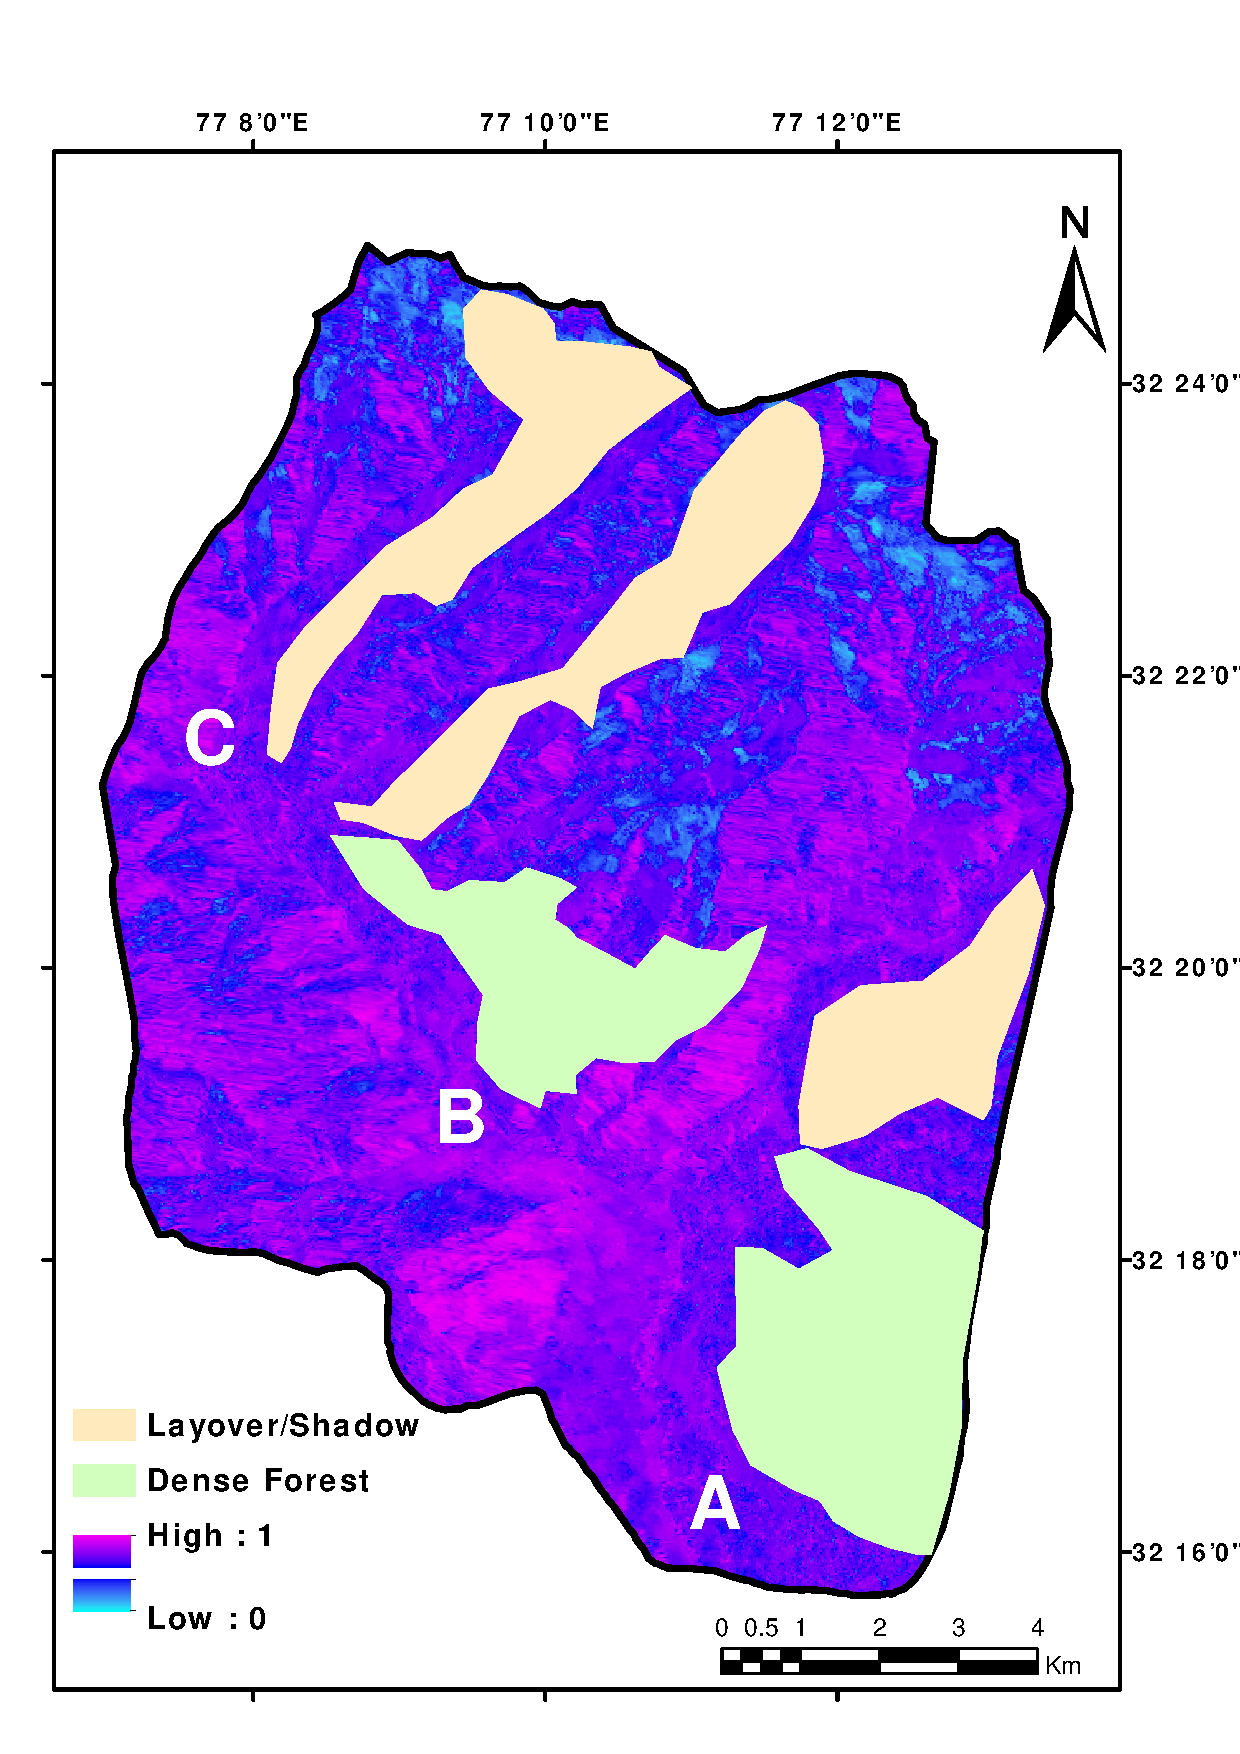
\includegraphics[width=0.4\columnwidth]{Figures_SSD/Ag4U_DOP}} 
%	\hspace{1mm}
%	\subfloat[$p_{max}$\label{Fig:Touzi_DOP}]{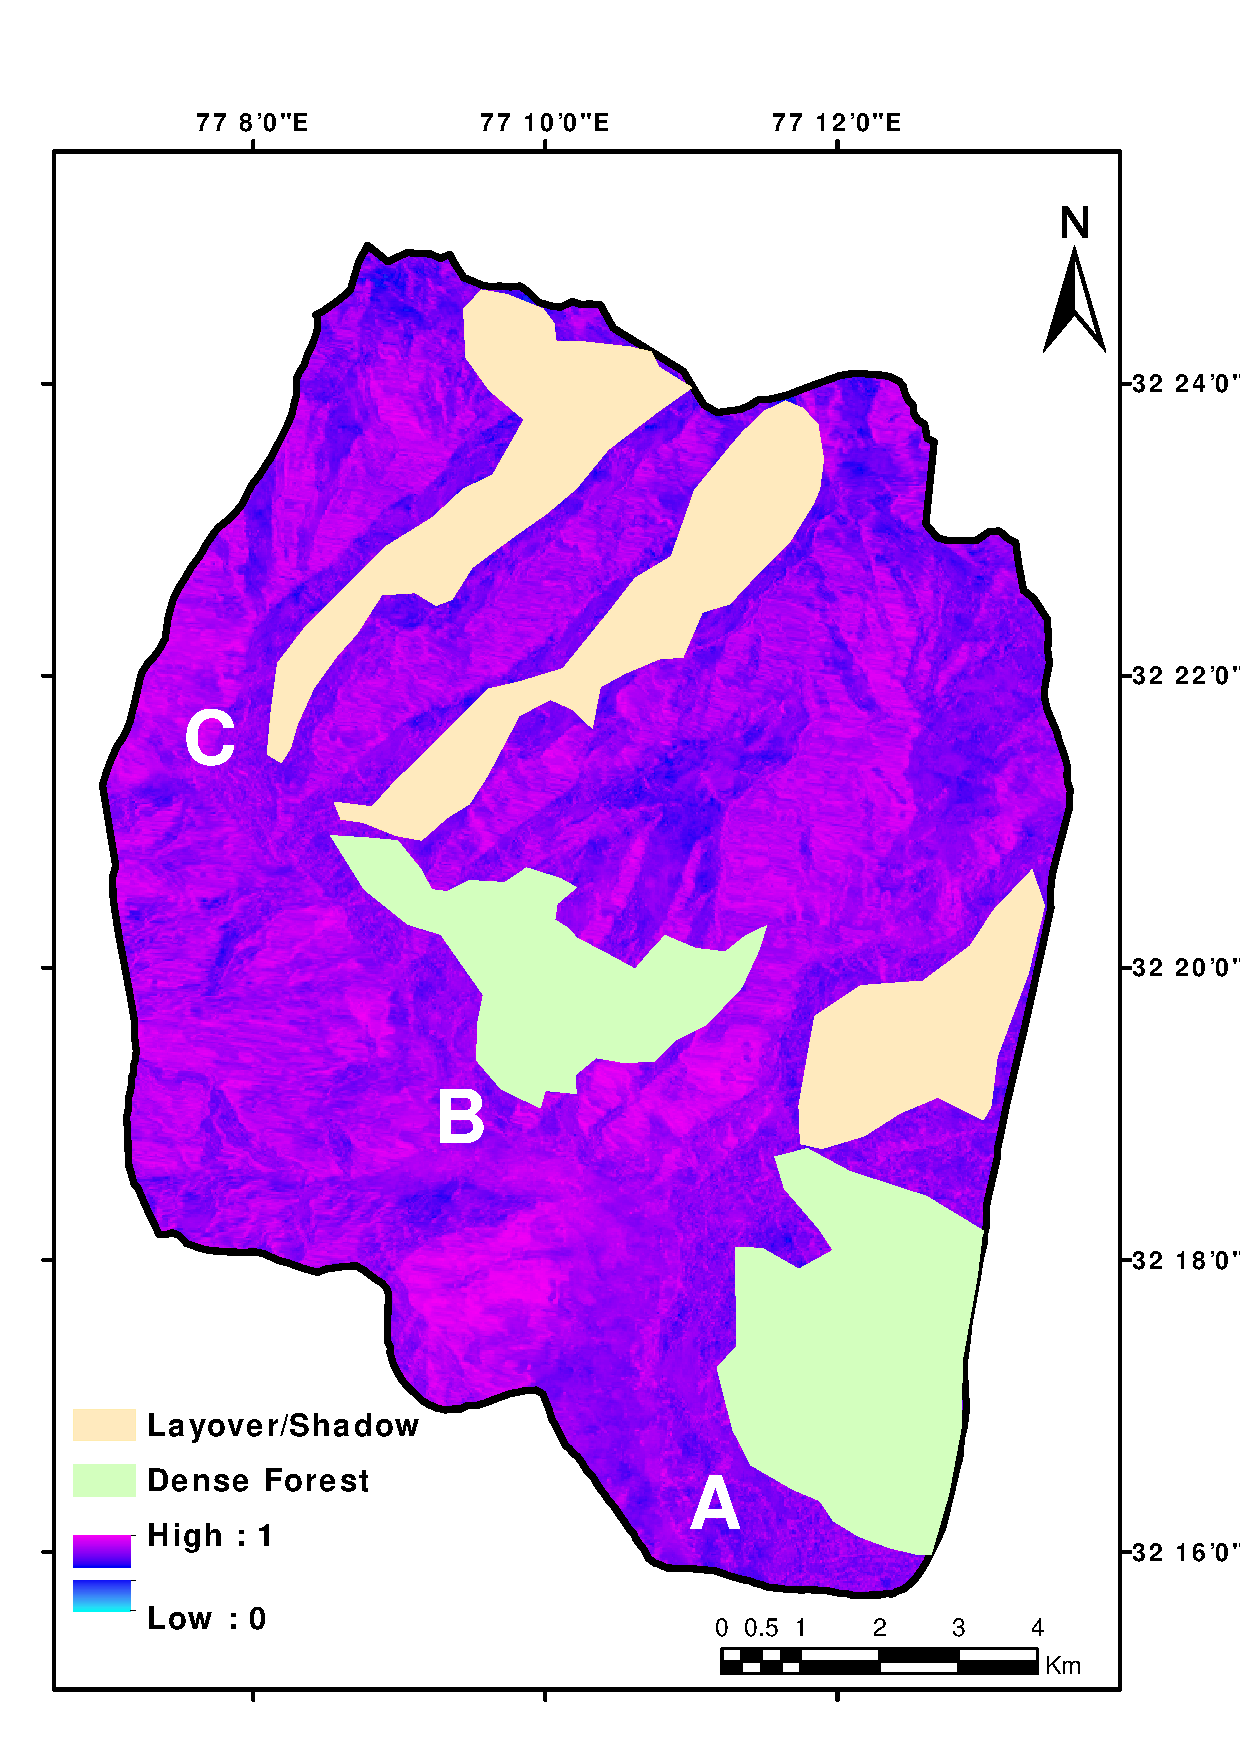
\includegraphics[width=0.4\columnwidth]{Figures_SSD/Touzi_DOP}} 
%	\vspace{1mm}
%	\subfloat[$\alpha_{s1}$\label{Fig:alpha_s1}]{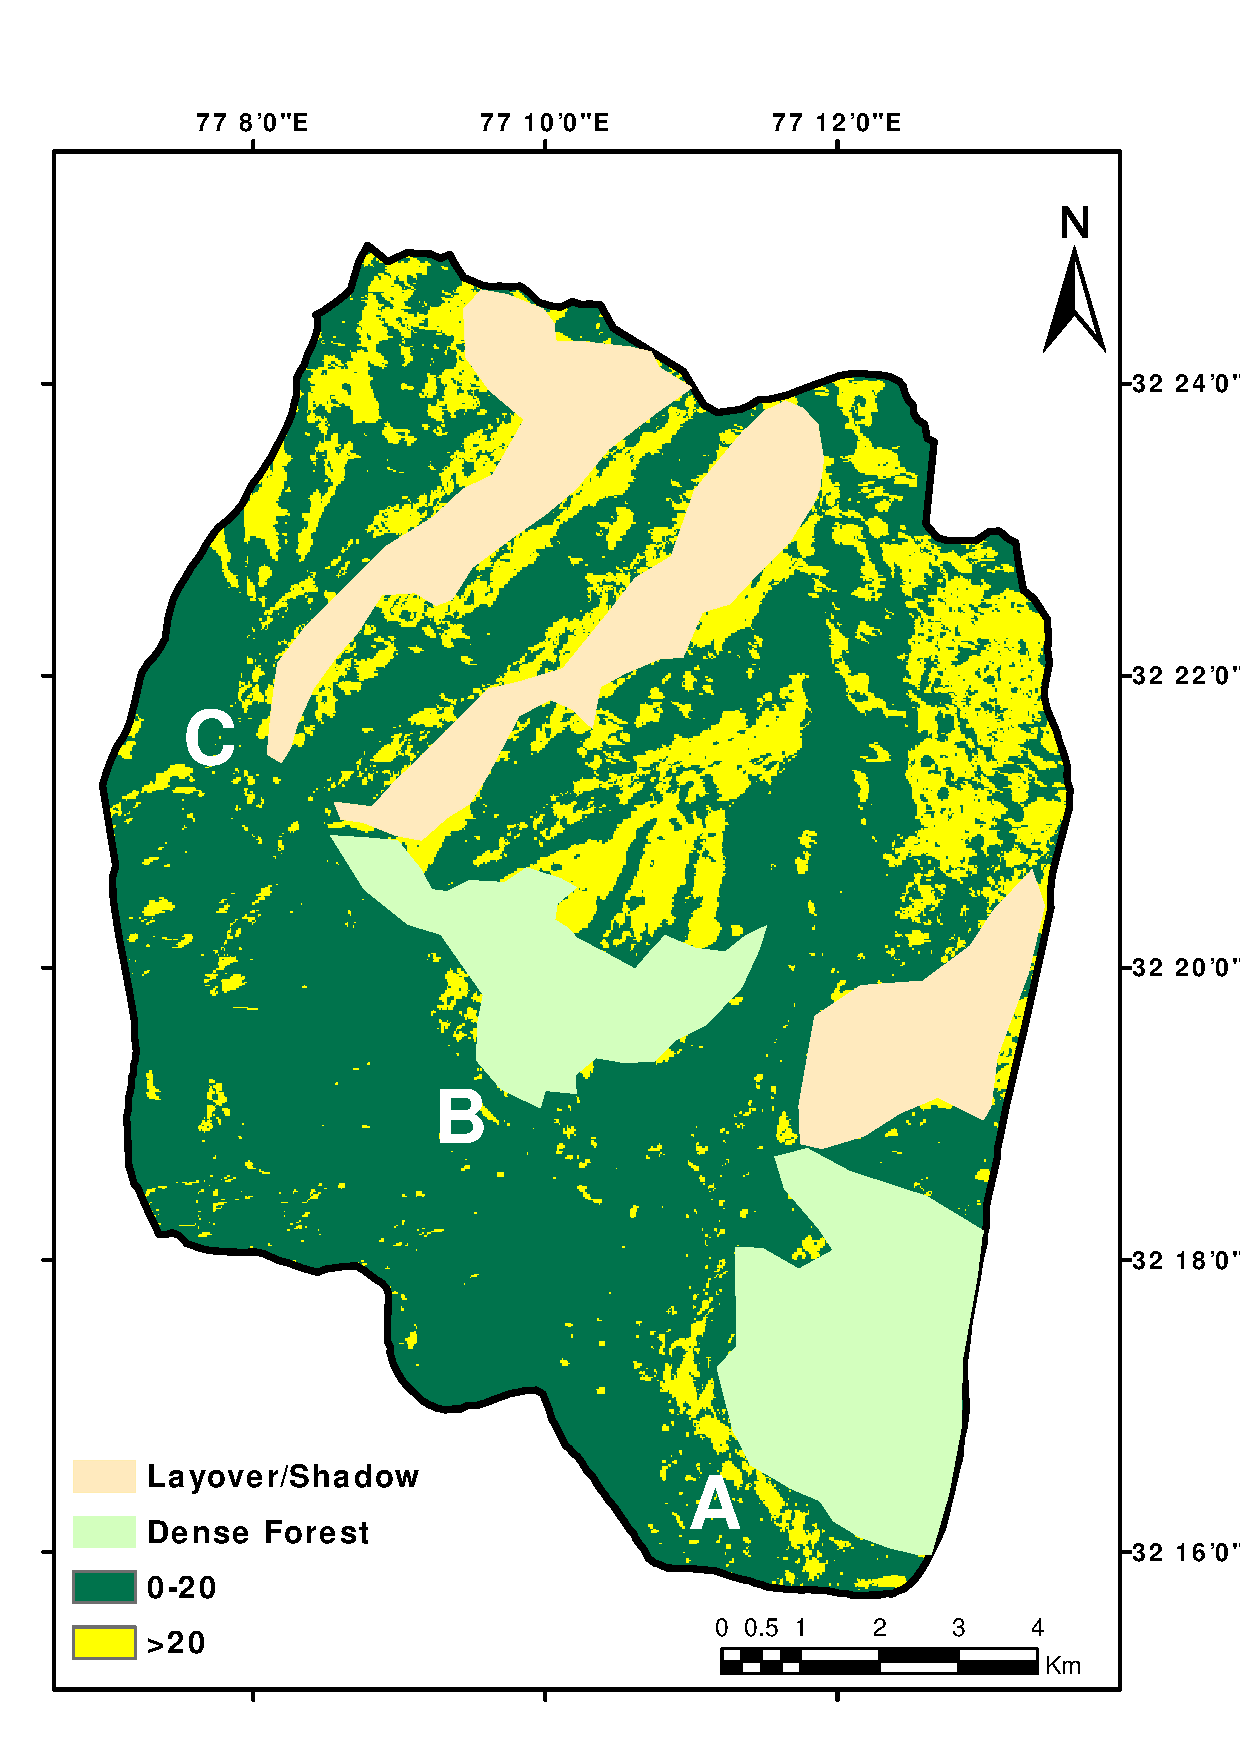
\includegraphics[width=0.4\columnwidth]{Figures_SSD/alpha_8feb13}} \hspace{1mm}
%	\subfloat[$\alpha_{s1} \mbox{vs.} Dop$\label{Fig:dop_alpha}]{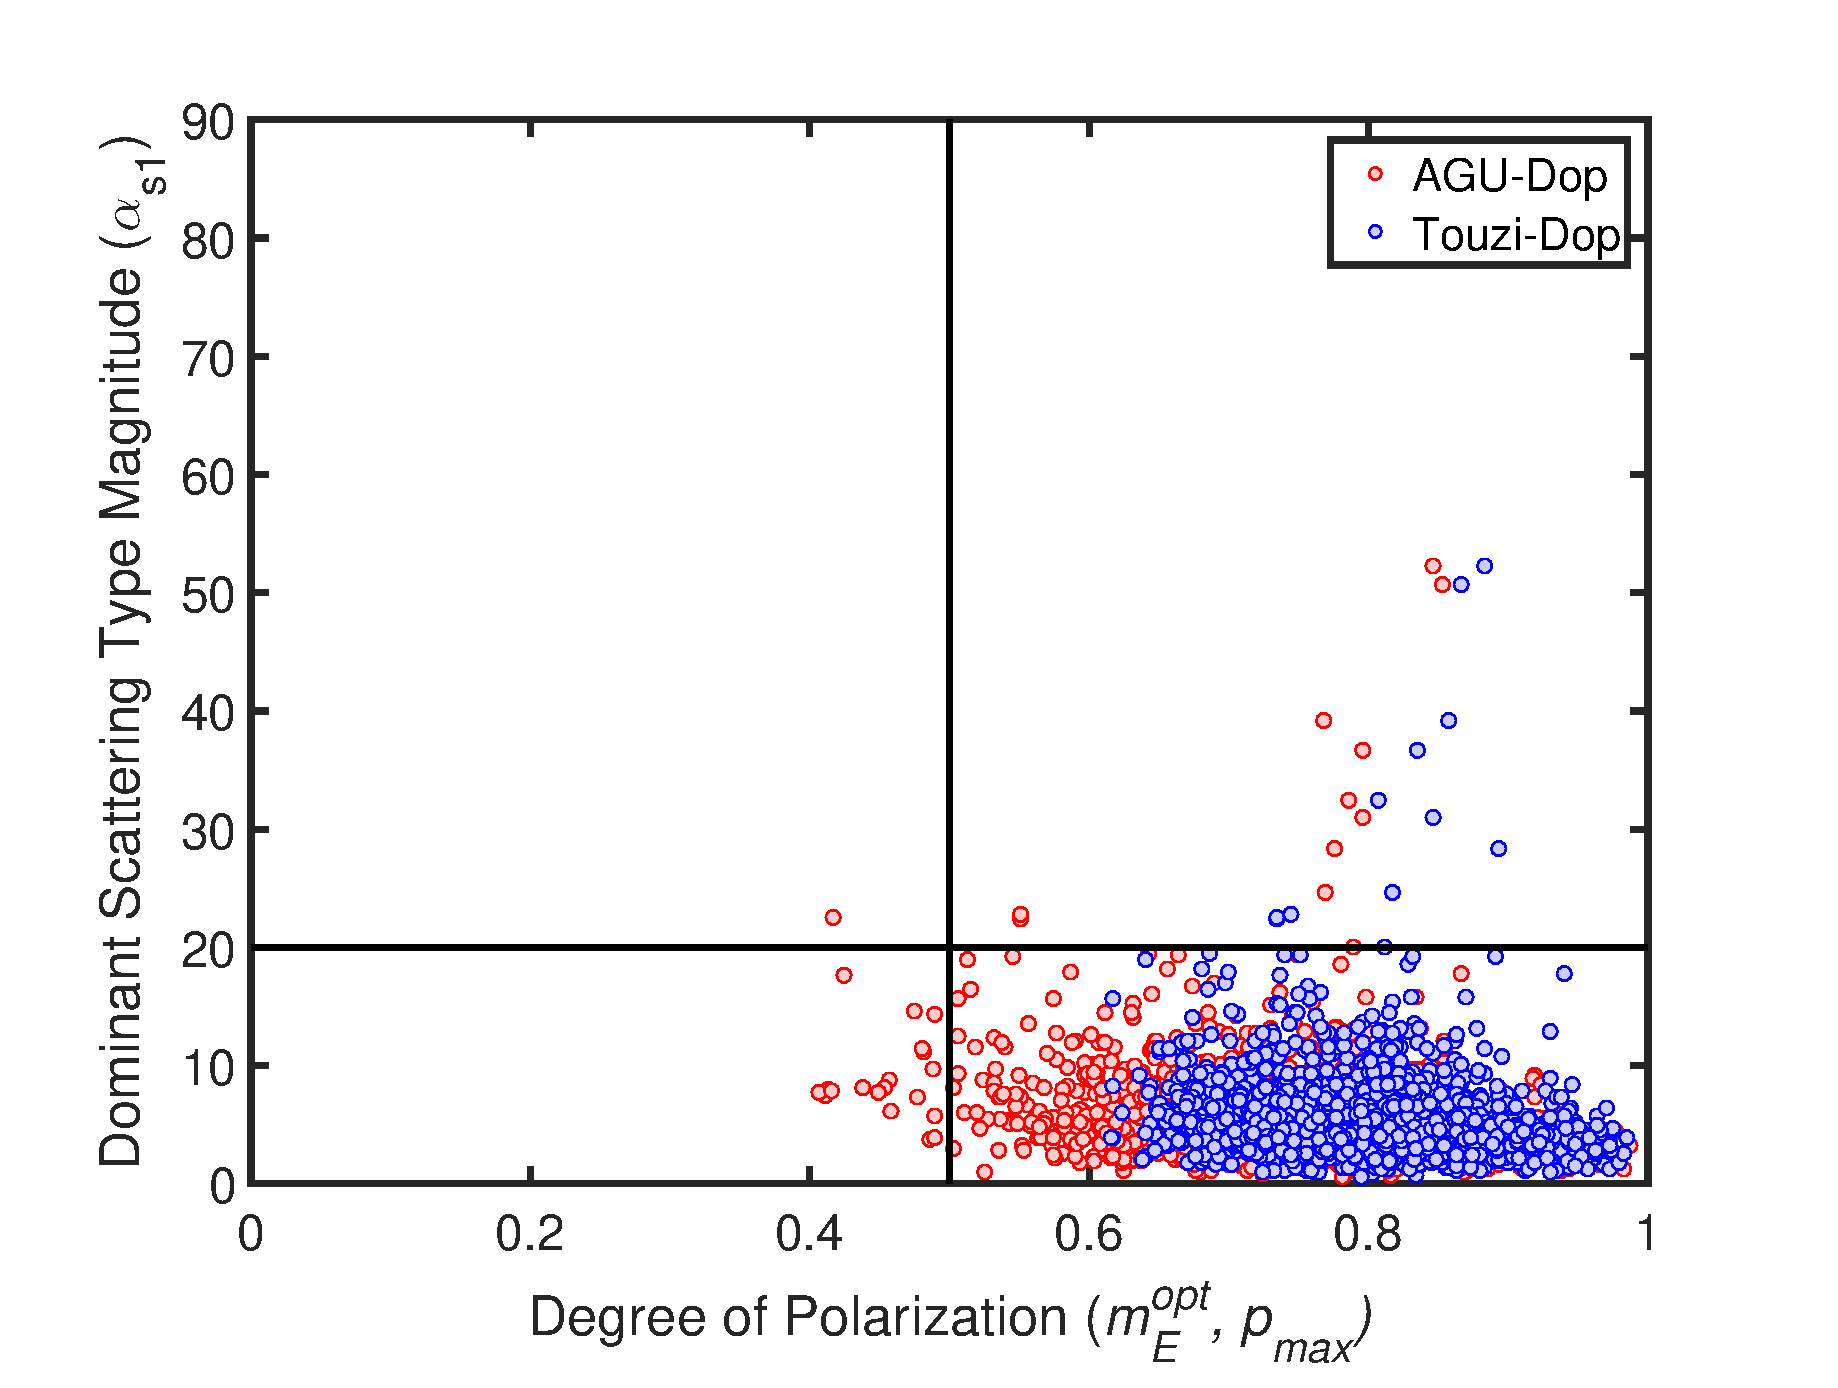
\includegraphics[width=0.4\columnwidth]{Figures_SSD/dop_alpha_1}} 
%	\caption[The optimum degree of polarization by (a) AGU and (b) Touzi methods, (c) The dominant scattering type magnitude (d) the $\alpha_{s1} \mbox{vs.} m_{E}^{\mbox{\scriptsize opt}}$ plot for 8 Feb.2013 data]{The optimum degree of polarization by (a) AGU and (b) Touzi methods, (c) The dominant scattering type magnitude (d) the $\alpha_{s1} \mbox{vs.} m_{E}^{\mbox{\scriptsize opt}}$ plot for 8 Feb.2013 data. The points A, B and C on the maps are the three observatory locations over the study area.}
%	\label{fig:results_1}
%\end{figure*}

\subsection{Snow surface dielectric constant}
The small perturbation or Bragg rough surface scattering~\citep{tsang1985theory} is defined for large (compared to the incident wavelength $\lambda$) surface facets where the rms surface roughness $s$ is small compared to $\lambda$. This is usually expressed in terms of the wavenumber $k$ and for all practical applications $ks < 0.3$. The backscattered power depends only on a certain frequency component which pertains to the surface roughness spectrum (the Fourier transform of the surface profile). Moreover, the surface roughness is implicit in the Fourier transform of the surface profile and it is similar to both the polarization channels (HH and VV). Hence, a simple ratio of the co-polarized channels (eg. HH/VV) will be only a function of the local incidence angle $\theta_{i}$ and the snow surface dielectric constant $\varepsilon_{r}$~\citep{cloude2009polarisation}. 

The Bragg scattering is considered without the cross-polarization component. The surface roughness criteria in this case is tightly constrained which limits its practical  applicability. In order to circumvent this problem, the extended Bragg (X-Bragg) model was proposed in~\cite{Hajnsek2003}. The scattered field ($\mathbf{E_{pq}^s}$) given in \eqref{eq:scattered_field} is related to the Bragg coefficients $B_{HH}$ and $B_{VV}$ for the co-polarized components~\eqref{eq:bragg_coefficients_1}--~\eqref{eq:bragg_coefficients_2}. These co-polarized components depend only on the local incidence angle $\theta$ and the dielectric constant $\varepsilon_{r}$, whereas the cross-polarized component $B_{HV}=B_{VH}=0$. 
\begin{subequations}
	\begin{align}
	\mathbf{E_{pq}^s} = & i2k\cos\theta B_{pq}\hat{Z}(2k\sin\theta)
	\label{eq:scattered_field} \\
	B_{HH} = & \frac{\mbox{cos}\theta_{i} - \sqrt{\varepsilon_{r} - \mbox{sin}^2\theta_{i}}}{\mbox{cos}\theta_{i} + \sqrt{\varepsilon_{r} - \mbox{sin}^2\theta_{i}}} \label{eq:bragg_coefficients_1}\\
	B_{VV} = & (\varepsilon_{r}-1)\frac{\mbox{sin}^2\theta_{i} - \varepsilon_{r}(1 + \mbox{sin}^2\theta_{i})}{\left[\varepsilon_{r}\mbox{cos}\theta_{i} + \sqrt{\varepsilon_{r} - \mbox{sin}^2\theta_{i}}\right]^2} \label{eq:bragg_coefficients_2} 
	\end{align}
\end{subequations}

Using this model, two independent parameters: roughness index and the moisture index were derived~\citep{cloude2002new}. The roughness index is dependent on the dielectric constant and the angle of incidence, while the moisture index is independent of the roughness and the surface scattering amplitude. It only depends on the dielectric constant $\varepsilon_{r}$ and the angle of incidence $\theta$. The moisture index is used in this study which relates the roll-invariant dominant scattering type amplitude $\alpha_{s1}$ to the Bragg coefficients $B_{HH}$ and $B_{VV}$~\eqref{eq:alphas1_bragg}.
\begin{equation}
\alpha_{s1}=\tan^{-1}\Bigg(\Bigg|\frac{B_{HH}-B_{VV}}{B_{HH}+B_{VV}}\Bigg|\Bigg), \quad \alpha_{s1} \in \alpha_{s1}^{B}
\label{eq:alphas1_bragg}
\end{equation}
%\begin{subequations}
%	\begin{align}
%	B_{HH} =& \frac{\mbox{cos}\theta_{i} - \sqrt{\varepsilon_{r} - \mbox{sin}^2\theta_{i}}}{\mbox{cos}\theta_{i} + \sqrt{\varepsilon_{r} - \mbox{sin}^2\theta_{i}}} \label{eq:bragg_coefficients_1}\\
%	B_{VV} =& (\varepsilon_{r}-1)\frac{\mbox{sin}^2\theta_{i} - \varepsilon_{r}(1 + \mbox{sin}^2\theta_{i})}{\left[\varepsilon_{r}\mbox{cos}\theta_{i} + \sqrt{\varepsilon_{r} - \mbox{sin}^2\theta_{i}}\right]^2} \label{eq:bragg_coefficients_2}
%	\end{align}
%\end{subequations}

Following this, the snow surface dielectric constant $\varepsilon_{r}$ is numerically obtained by inverting~\eqref{eq:alphas1_bragg} for only those pixels which lie in the region of $\alpha_{s1}^{B}$ and $m_{E}^{\mbox{\scriptsize opt}} > 0.5$. This can be clearly seen in Figure~\ref{fig:results_1}(d) for samples from the study area used in this paper for the 8 Feb data. This methodology can be justified by the fact that approximately $9-10\%$ increase in the number of pixels have been obtained as compared to the original data $(\langle[{\mathbf{T}}]\rangle)$, for all the data sets used in this study by using the criteria of optimum degree of polarization $m_{E}^{\mbox{\scriptsize opt}}$. These pixels lie in the region of $\alpha_{s1}^{B}$ and have been correctly inverted to obtain $\varepsilon_{r}$. 

\section{Snow density estimation using full polarimetric SAR data}
\label{sec:3.4}
Followed by the snow wetness estimation from full polarimetry SAR data~\ref{sec:3.2}, here also the general four-component scattering power decomposition method (G4U)~\citep{singh13} is adopted to develop a new snow density estimation method. The G4U decomposition which is used in this study, has the added advantage of full utilization of the polarimetric coherency phase information provided by a full-polarimetric SAR data. Unlike the L-band data, the estimation of the snow density using C-band relies mainly on the scattering from the snowpack volume. Therefore, the generalized volume parameter is utilized in this study. It is then directly used to invert the snowpack dielectric constant. The effective snow dielectric constant is derived using the normalized volume scattering power, which is then used in a standard semi-empirical equation~\citep{looyenga1965dielectric} to estimate the snow density. 

%Unlike the Freeman-Durden decomposition (FDD)~\citep{freeman98}, the Yamaguchi 4-component decomposition (Y4O)~\citep{Yamaguchi05} and the Yamaguchi 4-component decomposition with rotation (Y4R)~\citep{YAMAGUCHI2011}, which only uses 55.5$\%$, 66.6$\%$ and 75$\%$ of the polarimetric phase information respectively whereas the G4U utilizes 100$\%$ of the polarimetric phase information which is implemented by a double unitary transformation of the coherency matrix~(\ref{eq:g4u_decomposition_1} and~\ref{eq:g4u_decomposition_2}), 
%
%\begin{subequations}
%\begin{multline}
% \left\langle\mathbf{[T(\theta)]}\right\rangle = \left[U(\theta)\right]\Bigl(f_{s}\left\langle\mathbf{[T]}\right\rangle_{surface} +  f_{d}\left\langle\mathbf{[T]}\right\rangle_{double} + f_v\left\langle\mathbf{[T]}\right\rangle_{vol} \\ + f_{c}\left\langle\mathbf{[T]}\right\rangle_{helix}\Bigr)\left[U(\theta)\right]^{\dagger}
%\label{eq:g4u_decomposition_1}
%\end{multline}
%\begin{equation}
%\left\langle\mathbf{[T(\phi)]}\right\rangle = \left[U(\phi)\right]\left\langle\mathbf{[T(\theta)]}\right\rangle\left[U(\phi)\right]^{\dagger} = \left[ \begin{array}{ccc}
%T_{11} & T_{12} & T_{13} \\
%T_{21} & T_{22} & 0 \\
%T_{31} & 0 & T_{33}
%\end{array}\right] 
%\label{eq:g4u_decomposition_2}
%\end{equation}
%\begin{equation}
%\left[U(\theta)\right] = \left[ \begin{array}{ccc}
%1 & 0 & 0 \\
%0 & \mbox{cos}2\theta & \mbox{sin}2\theta \\
%0 & -\mbox{sin}2\theta & \mbox{cos}2\theta
%\end{array}\right];  \quad
%\left[U(\phi)\right] = \left[ \begin{array}{ccc}
%1 & 0 & 0 \\
%0 & \mbox{cos}2\phi & j\mbox{sin}2\phi \\
%0 & j\mbox{sin}2\phi & \mbox{cos}2\phi
%\end{array}\right]
%\label{eq:utheta_and_uphi}
%\end{equation}
%\end{subequations}
%where $\dagger$ denotes complex conjugation and transposition, $\left[U(\theta)\right]$ and $\left[U(\phi)\right]$ denotes the real and the complex unitary transformation matrices respectively~(\ref{eq:utheta_and_uphi}) and $\left\langle\mathbf{[T(\theta)]}\right\rangle = \left[U(\theta)\right]\left\langle\mathbf{[T]}\right\rangle\left[U(\theta)\right]^{\dagger}$ denotes the measured coherency matrix after real orientation compensation. The $f_{s}$, $f_d$, $f_v$ and $f_{c}$ are the corresponding scattering coefficients of the expansion matrices, $\left\langle\mathbf{[T]}\right\rangle_{surface}$, $\left\langle\mathbf{[T]}\right\rangle_{double}$, $\left\langle\mathbf{[T]}\right\rangle_{vol}$ and $\left\langle\mathbf{[T]}\right\rangle_{helix}$ respectively. These coefficient are then used to estimate the surface ($P_s$), double-bounce ($P_d$), volume ($P_v$) and the helix ($P_c$) scattering powers. 
%In this work the scattering by snow particles is modeled in terms of their polarizability.The volume scattering matrix defined for a single particle is defined as,
%\begin{equation}
%[S_{vol}]=\left[\begin{array}{cc}
%S_{HH}^{vol} & 0 \\
%0 & S_{VV}^{vol}
%\end{array}\right] = S_{HH}^{vol}\left[\begin{array}{cc}
%1 & 0 \\
%0 & A_{p}
%\end{array}\right]
%\label{eq:scattering_matrix_fung_sd}
%\end{equation}
%where $A_{p}$ is known as the particle anisotropy.The anisotropy can also be interpreted in terms of the particle geometry and can be defined as the ratio of the principal values of polarizability~\cite{cloude2009polarisation}. In general, the anisotropy parameter can be used to a certain degree of reliability as a reference for the particle shape. However, the anisotropy parameter is also bounded by the dielectric constant ($\varepsilon$) of the particle and is bounded by,
%\begin{equation}
%\frac{1}{\varepsilon{'}_{v}}<A_{p}<\frac{\varepsilon{'}_{v} + 1}{2}.
%\label{eq:anisotropy_sd}
%\end{equation}
%In order to have a volume scattering from a random cloud of snow particles, the volume scattering matrix defined in~(\ref{eq:scattering_matrix_fung_sd}) should be arbitrarily rotated about the line of sight by an angle $\theta$ as,
%\begin{equation}
%[S_{vol}]=S_{HH}^{vol}\left[\begin{array}{cc}
%\mbox{cos}(\theta) & \mbox{sin}(\theta) \\
%-\mbox{sin}(\theta) & \mbox{cos}(\theta)
%\end{array}\right]\left[\begin{array}{cc}
%1 & 0 \\
%0 & A_{p}
%\end{array}\right]\left[\begin{array}{cc}
%\mbox{cos}(\theta) & -\mbox{sin}(\theta) \\
%\mbox{sin}(\theta) & \mbox{cos}(\theta)
%\end{array}\right].
%\label{eq:rotated_volume_scattering_matrix_sd}
%\end{equation}
%for which the volume coherency matrix $[T(\theta)]_{vol}$ can be written as,
%\begin{equation}
%[T(\theta)]_{vol}=\frac{1}{2}\left|S_{HH}^{vol}\right|^2\left[\begin{array}{ccc}
%|1+A_{p}|^2 & (1 + A_{p})\mbox{cos}2\theta & -(1 + A_{p})\mbox{sin}2\theta    \\
%(1 + A_{p})^*\mbox{cos}2\theta & |1-A_{p}|^2\mbox{cos}^22\theta  & -|1-A_{p}|^2\frac{\mbox{sin}4\theta}{2}   \\ 
%-(1 + A_{p})^*\mbox{sin}2\theta & -|1-A_{p}|^2\frac{\mbox{sin}4\theta}{2} & |1-A_{p}|^2\mbox{sin}^22\theta
%\end{array}\right].
%\label{eq:coh_matrix_sp_sd}
%\end{equation}
%The volume scattering coherency matrix in~(\ref{eq:coh_matrix_sp_sd}) is averaged over all possible angles $\theta$ to obtain the volume scattering coherency matrix of a random cloud of small spheroid particles in one resolution cell as,
%\begin{equation}
%\left\langle[T]\right\rangle_{vol}^{snow}=\int[T(\theta)]_{vol}p(\theta)d\theta
%\label{eq:average_coherency_matrix_sd}
%\end{equation}
%for uniformly distributed snow particles, 
%\begin{equation}
%p(\theta)=\frac{1}{2\pi} \quad; 0<\theta<2\pi
%\label{eq:uniform_distrbn_sd}
%\end{equation}
%The average snow volume coherency matrix~(\ref{eq:volume_coherency_matrix_sd}) can be written in terms of generalized volume parameter ($|\gamma|^2$), 
%\begin{equation}
%\left\langle\mathbf{[T]}\right\rangle_{vol}^{snow} = f_{v}\left[ \begin{array}{ccc}
%|\gamma|^{2} & 0 & 0 \\
%0 & \frac{1}{2} & 0 \\
%0 & 0 & \frac{1}{2}
%\end{array}\right].
%\label{eq:volume_coherency_matrix_sd}
%\end{equation}
%with the volume scattering coefficient as,
%\begin{equation}
%f_{v} = \frac{1}{2}|\gamma_{HH}-\gamma_{VV}|^{2}f(\theta_{i},\theta_{r},\omega,\tau,P)
%\label{eq:fv_sw}
%\end{equation}
%where $\theta_{i}$ and $\theta_{r}$ are the local incidence and refractive angles, $\omega=\kappa_{s}/\kappa_{e}$ is the snow volume albedo, defined as the ratio of the scattering $\kappa_{s}$ and the extinction coefficient $\kappa_{e}$, $\tau$ is the optical depth ($\tau=\kappa_{e}d$) where $d$ is the snow depth, $P$ is the Rayleigh scattering phase function and,
%\begin{equation}
%|\gamma|^2 = \frac{|\gamma_{HH} + \gamma_{VV}|^2}{|\gamma_{HH} - \gamma_{VV}|^2} = \frac{|1 + A_{p}|^2}{|1 - A_{p}|^2}.
%\label{eq:gammasquare_sd}
%\end{equation}
%where $\gamma_{HH}$ and $\gamma_{VV}$ are the Fresnel transmission coefficients for HH and VV polarizations respectively,
%\begin{subequations}
%	\begin{align}
%	\gamma_{HH} =& \frac{2\sqrt{\varepsilon{'}_{v} - \mbox{sin}^2\theta_{i}}}{\mbox{cos}\theta_{i} + \sqrt{\varepsilon{'}_{v} - \mbox{sin}^2\theta_{i}}} \\
%	\gamma_{VV} =& \frac{2\sqrt{\varepsilon{'}_{v} - \mbox{sin}^2\theta_{i}}}{\varepsilon{'}_{v}\mbox{cos}\theta_{i} + \sqrt{\varepsilon{'}_{v} - \mbox{sin}^2\theta_{i}}}
%	\end{align}
%	\label{eq:fresnel_trans_coefficients_sd}
%\end{subequations}
%the local incidence angle $\theta_{i}$ should be converted into the local refractive angle $\theta_{r}$ using the Snell's law.
%%Since $A_{p}$ is bounded, therefore $|\gamma|^2$ is also bounded as,
%%\begin{equation}
%%\left|\frac{\varepsilon_{v}+1}{\varepsilon_{v}-1}\right|^2 < |\gamma|^2 < \left|\frac{\varepsilon_{v}+3}{\varepsilon_{v}-1}\right|^2
%%\end{equation}
%By assuming that the double-bounce scattering is negligible in wet snow, the generalized volume parameter $|\gamma|^2$ is derived~\cite{singh2013b} as,
%\begin{equation}
%|\gamma|^2 = \frac{T_{11}(\theta)}{2T_{33}(\theta)-f_c} - \frac{|T_{12}(\theta)+T_{13}(\theta)|^{2}}{(2T_{33}(\theta)-f_{c})(T_{22}(\theta)-T_{33}(\theta)}
%\label{eq:gamma_square_coherency_elememts_sd}
%\end{equation}
%where $f_{c}$ is the helix scattering coefficient given as,
%\begin{equation}
%f_{c}=2|\mbox{Im}\{T_{23}(\theta)\}|.
%\label{eq:helix_scattering_coefficient_sd}
%\end{equation}
%The snow volume dielectric constant is then estimated by equating~(\ref{eq:gammasquare_sd}) and~(\ref{eq:gamma_square_coherency_elememts_sd}).
The generalized volume parameter ($|\gamma|^2$) derived from~(\ref{eq:gamma_square_coherency_elememts_sw}) is equated with~(\ref{eq:gammasquare_sw}) for the inversion of snowpack volume dielectric constant. The estimated snowpack volume dielectric constant is normalized with the volume scattering power ($\omega=P_v/TP$) estimated from the G4U decomposition. This normalized (effective) snowpack dielectric constant ($\varepsilon_{e}{'}=\omega.\varepsilon_{v}{'}$) is then used in the Looyenga's semi-empirical dielectric equation~\citep{looyenga1965dielectric} to estimate the snow density ($\rho_s$). The flowchart of the proposed methodology is shown in Figure~\ref{fig:methodology}. 

\begin{equation}
\varepsilon_{e}{'}=1.0 + 1.5995\rho_s + 1.861\rho_s^{3}
\label{eq:looyenga}
\end{equation}

\begin{sidewaysfigure}
	\centering
	\includegraphics[width=0.49\textwidth]{Figures_sd/flow_chart}
	\caption [Flowchart of snow density estimation algorithm]{Flowchart of the snow density estimation method for C-band full polarimetric data}
	\label{fig:methodology}
\end{sidewaysfigure}

In this proposed method, the generalized volume parameter utilizes the full-polarimetric SAR measurements from the snowpack. Hence, this parameter is able to take care of various snow conditions. On the other hand, the scattering powers from the snowpack volume is a function of the penetration depth, the grain size, the snow wetness, etc. So, the generalized volume parameter combined with the scattering power is able to correctly quantify the snowpack density. During February, in the Indian Himalayan region, more than 90 $\%$ of the study area was completely covered with snow and our method was directly applied to the area. There was no masking used in this study to classify a area into wet/dry snow/snow free. The classification of wet or dry snow was not required because the proposed model takes into account different scattering mechanism contribution associated with different snow conditions while calculating the effective density.